\documentclass[10pt]{article}
\usepackage[utf8]{inputenc}
\usepackage[T1]{fontenc}
\usepackage{amsmath}
\usepackage{amsfonts}
\usepackage{amssymb}
\usepackage{mhchem}
\usepackage{stmaryrd}
\usepackage{bbold}
\usepackage{mathrsfs}
\usepackage{graphicx}
\usepackage[export]{adjustbox}
\graphicspath{ {./images/} }

\title{Chapter 4 }

\author{}
\date{}


\DeclareUnicodeCharacter{0131}{$\imath$}

\begin{document}
\maketitle
\section{Least Squares Regression}
\subsection{Introduction}
In this chapter we investigate some finite-sample properties of the least squares estimator in the linear regression model. In particular we calculate its finite-sample expectation and covariance matrix and propose standard errors for the coefficient estimators.

\subsection{Random Sampling}
Assumption $3.1$ specified that the observations have identical distributions. To derive the finitesample properties of the estimators we will need to additionally specify the dependence structure across the observations.

The simplest context is when the observations are mutually independent in which case we say that they are independent and identically distributed or i.i.d. It is also common to describe i.i.d. observations as a random sample. Traditionally, random sampling has been the default assumption in crosssection (e.g. survey) contexts. It is quite convenient as i.i.d. sampling leads to straightforward expressions for estimation variance. The assumption seems appropriate (meaning that it should be approximately valid) when samples are small and relatively dispersed. That is, if you randomly sample 1000 people from a large country such as the United States it seems reasonable to model their responses as mutually independent.

Assumption 4.1 The random variables $\left\{\left(Y_{1}, X_{1}\right), \ldots,\left(Y_{i}, X_{i}\right), \ldots,\left(Y_{n}, X_{n}\right)\right\}$ are independent and identically distributed.

For most of this chapter we will use Assumption $4.1$ to derive properties of the OLS estimator.

Assumption $4.1$ means that if you take any two individuals $i \neq j$ in a sample, the values $\left(Y_{i}, X_{i}\right)$ are independent of the values $\left(Y_{j}, X_{j}\right)$ yet have the same distribution. Independence means that the decisions and choices of individual $i$ do not affect the decisions of individual $j$ and conversely.

This assumption may be violated if individuals in the sample are connected in some way, for example if they are neighbors, members of the same village, classmates at a school, or even firms within a specific industry. In this case it seems plausible that decisions may be inter-connected and thus mutually dependent rather than independent. Allowing for such interactions complicates inference and requires specialized treatment. A currently popular approach which allows for mutual dependence is known as clustered dependence which assumes that that observations are grouped into "clusters" (for example, schools). We will discuss clustering in more detail in Section 4.21.

\subsection{Sample Mean}
We start with the simplest setting of the intercept-only model
$$
\begin{aligned}
Y &=\mu+e \\
\mathbb{E}[e] &=0 .
\end{aligned}
$$
which is equivalent to the regression model with $k=1$ and $X=1$. In the intercept model $\mu=\mathbb{E}[Y]$ is the expectation of $Y$. (See Exercise 2.15.) The least squares estimator $\widehat{\mu}=\bar{Y}$ equals the sample mean as shown in equation (3.8).

We now calculate the expectation and variance of the estimator $\bar{Y}$. Since the sample mean is a linear function of the observations its expectation is simple to calculate
$$
\mathbb{E}[\bar{Y}]=\mathbb{E}\left[\frac{1}{n} \sum_{i=1}^{n} Y_{i}\right]=\frac{1}{n} \sum_{i=1}^{n} \mathbb{E}\left[Y_{i}\right]=\mu .
$$
This shows that the expected value of the least squares estimator (the sample mean) equals the projection coefficient (the population expectation). An estimator with the property that its expectation equals the parameter it is estimating is called unbiased.

Definition $4.1$ An estimator $\widehat{\theta}$ for $\theta$ is unbiased if $\mathbb{E}[\widehat{\theta}]=\theta$

We next calculate the variance of the estimator $\bar{Y}$ under Assumption 4.1. Making the substitution $Y_{i}=\mu+e_{i}$ we find
$$
\bar{Y}-\mu=\frac{1}{n} \sum_{i=1}^{n} e_{i} .
$$
Then
$$
\begin{aligned}
\operatorname{var}[\bar{Y}] &=\mathbb{E}\left[(\bar{Y}-\mu)^{2}\right] \\
&=\mathbb{E}\left[\left(\frac{1}{n} \sum_{i=1}^{n} e_{i}\right)\left(\frac{1}{n} \sum_{j=1}^{n} e_{j}\right)\right] \\
&=\frac{1}{n^{2}} \sum_{i=1}^{n} \sum_{j=1}^{n} \mathbb{E}\left[e_{i} e_{j}\right] \\
&=\frac{1}{n^{2}} \sum_{i=1}^{n} \sigma^{2} \\
&=\frac{1}{n} \sigma^{2} .
\end{aligned}
$$
The second-to-last inequality is because $\mathbb{E}\left[e_{i} e_{j}\right]=\sigma^{2}$ for $i=j$ yet $\mathbb{E}\left[e_{i} e_{j}\right]=0$ for $i \neq j$ due to independence.

We have shown that $\operatorname{var}[\bar{Y}]=\frac{1}{n} \sigma^{2}$. This is the familiar formula for the variance of the sample mean.

\subsection{Linear Regression Model}
We now consider the linear regression model. Throughout this chapter we maintain the following.

\section{Assumption $4.2$ Linear Regression Model}
The variables $(Y, X)$ satisfy the linear regression equation
$$
\begin{aligned}
Y &=X^{\prime} \beta+e \\
\mathbb{E}[e \mid X] &=0 .
\end{aligned}
$$
The variables have finite second moments
$$
\begin{aligned}
&\mathbb{E}\left[Y^{2}\right]<\infty \\
&\mathbb{E}\|X\|^{2}<\infty
\end{aligned}
$$
and an invertible design matrix
$$
\boldsymbol{Q}_{X X}=\mathbb{E}\left[X X^{\prime}\right]>0 .
$$
We will consider both the general case of heteroskedastic regression where the conditional variance $\mathbb{E}\left[e^{2} \mid X\right]=\sigma^{2}(X)$ is unrestricted, and the specialized case of homoskedastic regression where the conditional variance is constant. In the latter case we add the following assumption.

\section{Assumption 4.3 Homoskedastic Linear Regression Model}
In addition to Assumption $4.2$
$$
\mathbb{E}\left[e^{2} \mid X\right]=\sigma^{2}(X)=\sigma^{2}
$$
is independent of $X$.

\subsection{Expectation of Least Squares Estimator}
In this section we show that the OLS estimator is unbiased in the linear regression model. This calculation can be done using either summation notation or matrix notation. We will use both.

First take summation notation. Observe that under (4.1)-(4.2)
$$
\mathbb{E}\left[Y_{i} \mid X_{1}, \ldots, X_{n}\right]=\mathbb{E}\left[Y_{i} \mid X_{i}\right]=X_{i}^{\prime} \beta .
$$
The first equality states that the conditional expectation of $Y_{i}$ given $\left\{X_{1}, \ldots, X_{n}\right\}$ only depends on $X_{i}$ because the observations are independent across $i$. The second equality is the assumption of a linear conditional expectation. Using definition (3.11), the conditioning theorem (Theorem 2.3), the linearity of expectations, (4.4), and properties of the matrix inverse,
$$
\begin{aligned}
\mathbb{E}\left[\widehat{\beta} \mid X_{1}, \ldots, X_{n}\right] &=\mathbb{E}\left[\left(\sum_{i=1}^{n} X_{i} X_{i}^{\prime}\right)^{-1}\left(\sum_{i=1}^{n} X_{i} Y_{i}\right) \mid X_{1}, \ldots, X_{n}\right] \\
&=\left(\sum_{i=1}^{n} X_{i} X_{i}^{\prime}\right)^{-1} \mathbb{E}\left[\left(\sum_{i=1}^{n} X_{i} Y_{i}\right) \mid X_{1}, \ldots, X_{n}\right] \\
&=\left(\sum_{i=1}^{n} X_{i} X_{i}^{\prime}\right)^{-1} \sum_{i=1}^{n} \mathbb{E}\left[X_{i} Y_{i} \mid X_{1}, \ldots, X_{n}\right] \\
&=\left(\sum_{i=1}^{n} X_{i} X_{i}^{\prime}\right)^{-1} \sum_{i=1}^{n} X_{i} \mathbb{E}\left[Y_{i} \mid X_{i}\right] \\
&=\left(\sum_{i=1}^{n} X_{i} X_{i}^{\prime}\right)^{-1} \sum_{i=1}^{n} X_{i} X_{i}^{\prime} \beta \\
&=\beta .
\end{aligned}
$$
Now let's show the same result using matrix notation. (4.4) implies
$$
\mathbb{E}[\boldsymbol{Y} \mid \boldsymbol{X}]=\left(\begin{array}{c}
\vdots \\
\mathbb{E}\left[Y_{i} \mid \boldsymbol{X}\right] \\
\vdots
\end{array}\right)=\left(\begin{array}{c}
\vdots \\
X_{i}^{\prime} \beta \\
\vdots
\end{array}\right)=\boldsymbol{X} \beta .
$$
Similarly
$$
\mathbb{E}[\boldsymbol{e} \mid \boldsymbol{X}]=\left(\begin{array}{c}
\vdots \\
\mathbb{E}\left[e_{i} \mid \boldsymbol{X}\right] \\
\vdots
\end{array}\right)=\left(\begin{array}{c}
\vdots \\
\mathbb{E}\left[e_{i} \mid X_{i}\right] \\
\vdots
\end{array}\right)=0 .
$$
Using $\widehat{\beta}=\left(\boldsymbol{X}^{\prime} \boldsymbol{X}\right)^{-1}\left(\boldsymbol{X}^{\prime} \boldsymbol{Y}\right)$, the conditioning theorem, the linearity of expectations, (4.5), and the properties of the matrix inverse,
$$
\begin{aligned}
\mathbb{E}[\widehat{\beta} \mid \boldsymbol{X}] &=\mathbb{E}\left[\left(\boldsymbol{X}^{\prime} \boldsymbol{X}\right)^{-1} \boldsymbol{X}^{\prime} \boldsymbol{Y} \mid \boldsymbol{X}\right] \\
&=\left(\boldsymbol{X}^{\prime} \boldsymbol{X}\right)^{-1} \boldsymbol{X}^{\prime} \mathbb{E}[\boldsymbol{Y} \mid \boldsymbol{X}] \\
&=\left(\boldsymbol{X}^{\prime} \boldsymbol{X}\right)^{-1} \boldsymbol{X}^{\prime} \boldsymbol{X} \beta \\
&=\beta .
\end{aligned}
$$
At the risk of belaboring the derivation, another way to calculate the same result is as follows. Insert $\boldsymbol{Y}=\boldsymbol{X} \beta+\boldsymbol{e}$ into the formula for $\widehat{\beta}$ to obtain
$$
\begin{aligned}
\widehat{\beta} &=\left(\boldsymbol{X}^{\prime} \boldsymbol{X}\right)^{-1}\left(\boldsymbol{X}^{\prime}(\boldsymbol{X} \beta+\boldsymbol{e})\right) \\
&=\left(\boldsymbol{X}^{\prime} \boldsymbol{X}\right)^{-1} \boldsymbol{X}^{\prime} \boldsymbol{X} \beta+\left(\boldsymbol{X}^{\prime} \boldsymbol{X}\right)^{-1}\left(\boldsymbol{X}^{\prime} \boldsymbol{e}\right) \\
&=\beta+\left(\boldsymbol{X}^{\prime} \boldsymbol{X}\right)^{-1} \boldsymbol{X}^{\prime} \boldsymbol{e} .
\end{aligned}
$$
This is a useful linear decomposition of the estimator $\widehat{\beta}$ into the true parameter $\beta$ and the stochastic component $\left(\boldsymbol{X}^{\prime} \boldsymbol{X}\right)^{-1} \boldsymbol{X}^{\prime} \boldsymbol{e}$. Once again, we can calculate that
$$
\begin{aligned}
\mathbb{E}[\widehat{\beta}-\beta \mid \boldsymbol{X}] &=\mathbb{E}\left[\left(\boldsymbol{X}^{\prime} \boldsymbol{X}\right)^{-1} \boldsymbol{X}^{\prime} \boldsymbol{e} \mid \boldsymbol{X}\right] \\
&=\left(\boldsymbol{X}^{\prime} \boldsymbol{X}\right)^{-1} \boldsymbol{X}^{\prime} \mathbb{E}[\boldsymbol{e} \mid \boldsymbol{X}]=0 .
\end{aligned}
$$
Regardless of the method we have shown that $\mathbb{E}[\widehat{\beta} \mid \boldsymbol{X}]=\beta$. We have shown the following theorem.

\section{Theorem 4.1 Expectation of Least Squares Estimator}
In the linear regression model (Assumption 4.2) with i.i.d. sampling (Assumption 4.1)
$$
\mathbb{E}[\widehat{\beta} \mid \boldsymbol{X}]=\beta .
$$
Equation (4.7) says that the estimator $\widehat{\beta}$ is unbiased for $\beta$, conditional on $\boldsymbol{X}$. This means that the conditional distribution of $\widehat{\beta}$ is centered at $\beta$. By "conditional on $X$ " this means that the distribution is unbiased for any realization of the regressor matrix $\boldsymbol{X}$. In conditional models we simply refer to this as saying $" \widehat{\beta}$ is unbiased for $\beta$ ".

It is worth mentioning that Theorem 4.1, and all finite sample results in this chapter, make the implicit assumption that $\boldsymbol{X}^{\prime} \boldsymbol{X}$ is full rank with probability one.

\subsection{Variance of Least Squares Estimator}
In this section we calculate the conditional variance of the OLS estimator.

For any $r \times 1$ random vector $Z$ define the $r \times r$ covariance matrix
$$
\operatorname{var}[Z]=\mathbb{E}\left[(Z-\mathbb{E}[Z])(Z-\mathbb{E}[Z])^{\prime}\right]=\mathbb{E}\left[Z Z^{\prime}\right]-(\mathbb{E}[Z])(\mathbb{E}[Z])^{\prime}
$$
and for any pair $(Z, X)$ define the conditional covariance matrix
$$
\operatorname{var}[Z \mid X]=\mathbb{E}\left[(Z-\mathbb{E}[Z \mid X])(Z-\mathbb{E}[Z \mid X])^{\prime} \mid X\right] .
$$
We define $\boldsymbol{V}_{\widehat{\beta}} \stackrel{\text { def }}{=} \operatorname{var}[\widehat{\beta} \mid \boldsymbol{X}]$ as the conditional covariance matrix of the regression coefficient estimators. We now derive its form.

The conditional covariance matrix of the $n \times 1$ regression error $\boldsymbol{e}$ is the $n \times n$ matrix
$$
\operatorname{var}[\boldsymbol{e} \mid \boldsymbol{X}]=\mathbb{E}\left[\boldsymbol{e} \boldsymbol{e}^{\prime} \mid \boldsymbol{X}\right] \stackrel{\text { def }}{=} \boldsymbol{D} .
$$
The $i^{t h}$ diagonal element of $\boldsymbol{D}$ is
$$
\mathbb{E}\left[e_{i}^{2} \mid \boldsymbol{X}\right]=\mathbb{E}\left[e_{i}^{2} \mid X_{i}\right]=\sigma_{i}^{2}
$$
while the $i j^{t h}$ off-diagonal element of $\boldsymbol{D}$ is
$$
\mathbb{E}\left[e_{i} e_{j} \mid \boldsymbol{X}\right]=\mathbb{E}\left(e_{i} \mid X_{i}\right) \mathbb{E}\left[e_{j} \mid X_{j}\right]=0
$$
where the first equality uses independence of the observations (Assumption 4.1) and the second is (4.2). Thus $\boldsymbol{D}$ is a diagonal matrix with $i^{t h}$ diagonal element $\sigma_{i}^{2}$ :
$$
\boldsymbol{D}=\operatorname{diag}\left(\sigma_{1}^{2}, \ldots, \sigma_{n}^{2}\right)=\left(\begin{array}{cccc}
\sigma_{1}^{2} & 0 & \cdots & 0 \\
0 & \sigma_{2}^{2} & \cdots & 0 \\
\vdots & \vdots & \ddots & \vdots \\
0 & 0 & \cdots & \sigma_{n}^{2}
\end{array}\right)
$$
In the special case of the linear homoskedastic regression model (4.3), then $\mathbb{E}\left[e_{i}^{2} \mid X_{i}\right]=\sigma_{i}^{2}=\sigma^{2}$ and we have the simplification $\boldsymbol{D}=\boldsymbol{I}_{n} \sigma^{2}$. In general, however, $\boldsymbol{D}$ need not necessarily take this simplified form.

For any $n \times r$ matrix $\boldsymbol{A}=\boldsymbol{A}(\boldsymbol{X})$,
$$
\operatorname{var}\left[\boldsymbol{A}^{\prime} \boldsymbol{Y} \mid \boldsymbol{X}\right]=\operatorname{var}\left[\boldsymbol{A}^{\prime} \boldsymbol{e} \mid \boldsymbol{X}\right]=\boldsymbol{A}^{\prime} \boldsymbol{D} \boldsymbol{A} .
$$
In particular, we can write $\widehat{\beta}=\boldsymbol{A}^{\prime} \boldsymbol{Y}$ where $\boldsymbol{A}=\boldsymbol{X}\left(\boldsymbol{X}^{\prime} \boldsymbol{X}\right)^{-1}$ and thus
$$
\boldsymbol{V}_{\widehat{\beta}}=\operatorname{var}[\widehat{\beta} \mid \boldsymbol{X}]=\boldsymbol{A}^{\prime} \boldsymbol{D} \boldsymbol{A}=\left(\boldsymbol{X}^{\prime} \boldsymbol{X}\right)^{-1} \boldsymbol{X}^{\prime} \boldsymbol{D} \boldsymbol{X}\left(\boldsymbol{X}^{\prime} \boldsymbol{X}\right)^{-1} .
$$
It is useful to note that
$$
\boldsymbol{X}^{\prime} \boldsymbol{D} \boldsymbol{X}=\sum_{i=1}^{n} X_{i} X_{i}^{\prime} \sigma_{i}^{2},
$$
a weighted version of $\boldsymbol{X}^{\prime} \boldsymbol{X}$.

In the special case of the linear homoskedastic regression model, $\boldsymbol{D}=\boldsymbol{I}_{n} \sigma^{2}$, so $\boldsymbol{X}^{\prime} \boldsymbol{D} \boldsymbol{X}=\boldsymbol{X}^{\prime} \boldsymbol{X} \sigma^{2}$, and the covariance matrix simplifies to $\boldsymbol{V}_{\widehat{\beta}}=\left(\boldsymbol{X}^{\prime} \boldsymbol{X}\right)^{-1} \sigma^{2}$.

\section{Theorem 4.2 Variance of Least Squares Estimator}
In the linear regression model (Assumption 4.2) with i.i.d. sampling (Assumption 4.1)
$$
\boldsymbol{V}_{\widehat{\beta}}=\operatorname{var}[\widehat{\beta} \mid \boldsymbol{X}]=\left(\boldsymbol{X}^{\prime} \boldsymbol{X}\right)^{-1}\left(\boldsymbol{X}^{\prime} \boldsymbol{D} \boldsymbol{X}\right)\left(\boldsymbol{X}^{\prime} \boldsymbol{X}\right)^{-1}
$$
where $\boldsymbol{D}$ is defined in (4.8). If in addition the error is homoskedastic (Assumption 4.3) then (4.10) simplifies to $\boldsymbol{V}_{\widehat{\beta}}=\sigma^{2}\left(\boldsymbol{X}^{\prime} \boldsymbol{X}\right)^{-1}$.

\subsection{Unconditional Moments}
The previous sections derived the form of the conditional expectation and variance of the least squares estimator where we conditioned on the regressor matrix $\boldsymbol{X}$. What about the unconditional expectation and variance?

Indeed, it is not obvious if $\widehat{\beta}$ has a finite expectation or variance. Take the case of a single dummy variable regressor $D_{i}$ with no intercept. Assume $\mathbb{P}\left[D_{i}=1\right]=p<1$. Then
$$
\widehat{\beta}=\frac{\sum_{i=1}^{n} D_{i} Y_{i}}{\sum_{i=1}^{n} D_{i}}
$$
is well defined if $\sum_{i=1}^{n} D_{i}>0$. However, $\mathbb{P}\left[\sum_{i=1}^{n} D_{i}=0\right]=(1-p)^{n}>0$. This means that with positive (but small) probability $\widehat{\beta}$ does not exist. Consequently $\widehat{\beta}$ has no finite moments! We ignore this complication in practice but it does pose a conundrum for theory. This existence problem arises whenever there are discrete regressors.

This dilemma is avoided when the regressors have continuous distributions. A clean statement was obtained by Kinal (1980) under the assumption of normal regressors and errors. Theorem 4.3 Kinal (1980)

In the linear regression model with i.i.d. sampling, if in addition $(X, e)$ have a joint normal distribution, then for any $r, \mathbb{E}\|\widehat{\beta}\|^{r}<\infty$ if and only if $r<n-k+1$.

This shows that when the errors and regressors are normally distributed that the least squares estimator possesses all moments up to $n-k$ which includes all moments of practical interest. The normality assumption is not critical for this result. What is key is the assumption that the regressors are continuously distributed.

The law of iterated expectations (Theorem 2.1) combined with Theorems $4.1$ and $4.3$ allow us to deduce that the least squares estimator is unconditionally unbiased. Under the normality assumption Theorem $4.3$ allows us to apply the law of iterated expectations, and thus using Theorems $4.1$ we deduce that if $n>k$
$$
\mathbb{E}[\widehat{\beta}]=\mathbb{E}[\mathbb{E}[\widehat{\beta} \mid \boldsymbol{X}]]=\beta .
$$
Hence $\widehat{\beta}$ is unconditionally unbiased as asserted.

Furthermore, if $n-k>1$ then $\mathbb{E}\|\widehat{\beta}\|^{2}<\infty$ and $\widehat{\beta}$ has a finite unconditional variance. Using Theorem $2.8$ we can calculate explicitly that
$$
\operatorname{var}[\widehat{\beta}]=\mathbb{E}[\operatorname{var}[\widehat{\beta} \mid \boldsymbol{X}]]+\operatorname{var}[\mathbb{E}[\widehat{\beta} \mid \boldsymbol{X}]]=\mathbb{E}\left[\left(\boldsymbol{X}^{\prime} \boldsymbol{X}\right)^{-1}\left(\boldsymbol{X}^{\prime} \boldsymbol{D} \boldsymbol{X}\right)\left(\boldsymbol{X}^{\prime} \boldsymbol{X}\right)^{-1}\right]
$$
the second equality because $\mathbb{E}[\widehat{\beta} \mid \boldsymbol{X}]=\beta$ has zero variance. In the homoskedastic case this simplifies to
$$
\operatorname{var}[\widehat{\beta}]=\sigma^{2} \mathbb{E}\left[\left(\boldsymbol{X}^{\prime} \boldsymbol{X}\right)^{-1}\right] .
$$
In both cases the expectation cannot pass through the matrix inverse because this is a nonlinear function. Thus there is not a simple expression for the unconditional variance, other than stating that is it the expectation of the conditional variance.

\subsection{Gauss-Markov Theorem}
The Gauss-Markov Theorem is one of the most celebrated results in econometric theory. It provides a classical justification for the least squares estimator, showing that it is lowest variance among unbiased estimators.

Write the homoskedastic linear regression model in vector format as
$$
\begin{aligned}
\boldsymbol{Y} &=\boldsymbol{X} \beta+\boldsymbol{e} \\
\mathbb{E}[\boldsymbol{e} \mid \boldsymbol{X}] &=0 \\
\operatorname{var}[\boldsymbol{e} \mid \boldsymbol{X}] &=\boldsymbol{I}_{n} \sigma^{2} .
\end{aligned}
$$
In this model we know that the least squares estimator is unbiased for $\beta$ and has covariance matrix $\sigma^{2}\left(\boldsymbol{X}^{\prime} \boldsymbol{X}\right)^{-1}$. The question raised in this section is if there exists an alternative unbiased estimator $\widetilde{\beta}$ which has a smaller covariance matrix.

The following version of the theorem is due to B. E. Hansen (2021).

\section{Theorem 4.4 Gauss-Markov}
Take the homoskedastic linear regression model (4.11)-(4.13). If $\widetilde{\beta}$ is an unbiased estimator of $\beta$ then
$$
\operatorname{var}[\widetilde{\beta} \mid \boldsymbol{X}] \geq \sigma^{2}\left(\boldsymbol{X}^{\prime} \boldsymbol{X}\right)^{-1}
$$
Theorem $4.4$ provides a lower bound on the covariance matrix of unbiased estimators under the assumption of homoskedasticity. It says that no unbiased estimator can have a variance matrix smaller (in the positive definite sense) than $\sigma^{2}\left(\boldsymbol{X}^{\prime} \boldsymbol{X}\right)^{-1}$. Since the variance of the OLS estimator is exactly equal to this bound this means that no unbiased estimator has a lower variance than OLS. Consequently we describe OLS as efficient in the class of unbiased estimators.

This earliest version of Theorem $4.4$ was articulated by Carl Friedrich Gauss in 1823. Andreı̆ Andreevich Markov provided a textbook treatment of the theorem in 1912, and clarified the central role of unbiasedness, which Gauss had only assumed implicitly.

Their versions of the Theorem restricted attention to linear estimators of $\beta$, which are estimators that can be written as $\widetilde{\beta}=\boldsymbol{A}^{\prime} \boldsymbol{Y}$, where $\boldsymbol{A}=\boldsymbol{A}(\boldsymbol{X})$ is an $m \times n$ function of the regressors $\boldsymbol{X}$. Linearity in this context means "linear in $\boldsymbol{Y}$ ". This restriction simplifies variance calculations, but greatly limits the class of estimators.This classical version of the Theorem gave rise to the description of OLS as the best linear unbiased estimator (BLUE). However, Theorem $4.4$ as stated above shows that OLS is the best unbiased estimator (BUE).

The derivation of the Gauss-Markov Theorem under the restriction to linear estimators is straightforward, so we now provide this demonstration. For $\widetilde{\beta}=\boldsymbol{A}^{\prime} \boldsymbol{Y}$ we have
$$
\mathbb{E}[\widetilde{\beta} \mid \boldsymbol{X}]=\boldsymbol{A}^{\prime} \mathbb{E}[\boldsymbol{Y} \mid \boldsymbol{X}]=\boldsymbol{A}^{\prime} \boldsymbol{X} \beta,
$$
the second equality because $\mathbb{E}[\boldsymbol{Y} \mid \boldsymbol{X}]=\boldsymbol{X} \beta$. Then $\widetilde{\beta}$ is unbiased for all $\beta$ if (and only if) $\boldsymbol{A}^{\prime} \boldsymbol{X}=\boldsymbol{I}_{k}$. Furthermore, we saw in (4.9) that
$$
\operatorname{var}[\widetilde{\beta} \mid \boldsymbol{X}]=\operatorname{var}\left[\boldsymbol{A}^{\prime} \boldsymbol{Y} \mid \boldsymbol{X}\right]=\boldsymbol{A}^{\prime} \boldsymbol{D} \boldsymbol{A}=\boldsymbol{A}^{\prime} \boldsymbol{A} \boldsymbol{\sigma}^{2}
$$
the last equality using the homoskedasticity assumption (4.13). To establish the Theorem we need to show that for any such matrix $\boldsymbol{A}$,
$$
\boldsymbol{A}^{\prime} \boldsymbol{A} \geq\left(\boldsymbol{X}^{\prime} \boldsymbol{X}\right)^{-1} \text {. }
$$
Set $\boldsymbol{C}=\boldsymbol{A}-\boldsymbol{X}\left(\boldsymbol{X}^{\prime} \boldsymbol{X}\right)^{-1}$. Note that $\boldsymbol{X}^{\prime} \boldsymbol{C}=0$. We calculate that
$$
\begin{aligned}
\boldsymbol{A}^{\prime} \boldsymbol{A}-\left(\boldsymbol{X}^{\prime} \boldsymbol{X}\right)^{-1} &=\left(\boldsymbol{C}+\boldsymbol{X}\left(\boldsymbol{X}^{\prime} \boldsymbol{X}\right)^{-1}\right)^{\prime}\left(\boldsymbol{C}+\boldsymbol{X}\left(\boldsymbol{X}^{\prime} \boldsymbol{X}\right)^{-1}\right)-\left(\boldsymbol{X}^{\prime} \boldsymbol{X}\right)^{-1} \\
&=\boldsymbol{C}^{\prime} \boldsymbol{C}+\boldsymbol{C}^{\prime} \boldsymbol{X}\left(\boldsymbol{X}^{\prime} \boldsymbol{X}\right)^{-1}+\left(\boldsymbol{X}^{\prime} \boldsymbol{X}\right)^{-1} \boldsymbol{X}^{\prime} \boldsymbol{C} \\
&+\left(\boldsymbol{X}^{\prime} \boldsymbol{X}\right)^{-1} \boldsymbol{X}^{\prime} \boldsymbol{X}\left(\boldsymbol{X}^{\prime} \boldsymbol{X}\right)^{-1}-\left(\boldsymbol{X}^{\prime} \boldsymbol{X}\right)^{-1} \\
&=\boldsymbol{C}^{\prime} \boldsymbol{C} \geq 0
\end{aligned}
$$
The final inequality states that the matrix $\boldsymbol{C}^{\prime} \boldsymbol{C}$ is positive semi-definite which is a property of quadratic forms (see Appendix A.10). We have shown (4.14) as required.

The above derivation imposed the restriction that the estimator $\widetilde{\beta}$ is linear in $\boldsymbol{Y}$. The proof of Theorem $4.4$ in the general case is considerably more advanced. Here, we provide a simplified sketch of the argument for interested readers, with a complete proof in Section 4.24. For simplicity, treat the regressors $X$ as fixed, and suppose that $Y$ has a density $f(y)$ with bounded support $\mathscr{Y}$. Without loss of generality assume that the true coefficient equals $\beta_{0}=0$.

Since $Y$ has bounded support $\mathscr{Y}$ there is a set $B \subset \mathbb{R}^{m}$ such that $\left|y X^{\prime} \beta / \sigma^{2}\right|<1$ for all $\beta \in B$ and $y \in \mathscr{Y}$. For such values of $\beta$, define the auxiliary density function
$$
f_{\beta}(y)=f(y)\left(1+y X^{\prime} \beta / \sigma^{2}\right) .
$$
Under the assumptions, $0 \leq f_{\beta}(y) \leq 2 f(y), f_{\beta}(y)$ has support $\mathscr{Y}$, and $\int_{\mathscr{Y}} f_{\beta}(y) d y=1$. To see the later, observe that $\int_{\mathscr{Y}} y f(y) d y=X^{\prime} \beta_{0}=0$ under the normalization $\beta_{0}=0$, and thus
$$
\int_{\mathscr{Y}} f_{\beta}(y) d y=\int_{\mathscr{Y}} f(y) d y+\int_{\mathscr{Y}} f(y) y d y X^{\prime} \beta / \sigma^{2}=1
$$
because $\int_{\mathscr{Y}} f(y) d y=1$. Thus $f_{\beta}$ is a parametric family of density functions. Evaluated at $\beta_{0}$ we see that $f_{0}=f$, which means that $f_{\beta}$ is a correctly-specified parametric family with true parameter value $\beta_{0}=0$.

To illustrate, take the case $X=1$. Figure 4.1 displays an example density $f(y)=(3 / 4)\left(1-y^{2}\right)$ on $[-1,1]$ with auxiliary density $f_{\beta}(y)=f(y)(1+y)$. We can see how the auxiliary density is a tilted version of the original density $f(y)$.

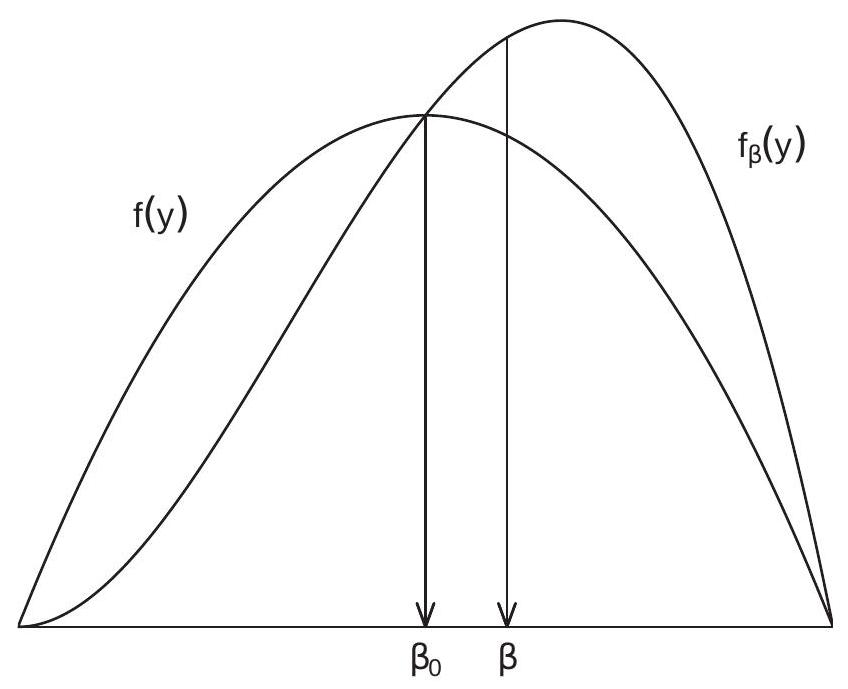
\includegraphics[max width=\textwidth]{2022_09_17_46fafb30295495354ae2g-09}

Figure 4.1: Original and Auxiliary Density

Let $\mathbb{E}_{\beta}$ denote expectation with respect to the auxiliary distribution. Since $\int_{\mathscr{Y}} y f(y) d y=0$ and $\int_{\mathscr{Y}} y^{2} f(y) d y=$ $\sigma^{2}$, we find
$$
\mathbb{E}_{\beta}[Y]=\int_{\mathscr{Y}} y f_{\beta}(y) d y=\int_{\mathscr{Y}} y f(y) d y+\int_{\mathscr{Y}} y^{2} f(y) d y X^{\prime} \beta / \sigma^{2}=X^{\prime} \beta .
$$
This shows that $f_{\beta}$ is a regression model with regression coefficient $\beta$.

In Figure 4.1, the means of the two densities are indicated by the arrows to the $\mathrm{x}$-axis. In this example we can see how the auxiliary density has a larger expected value, because the density has been tilted to the right.

The parametric family $f_{\beta}$ over $\beta \in B$ has the following properties: its expectation is $X^{\prime} \beta$, its variance is finite, the true value $\beta_{0}$ lies in the interior of $B$, and the support of the distribution does not depend on $\beta$.

The likelihood score of the auxiliary density function for an observation, using the fact that $Y_{i}=e_{i}$, is
$$
S_{i}=\left.\frac{\partial}{\partial \beta}\left(\log f_{\beta}\left(Y_{i}\right)\right)\right|_{\beta=0}=\left.\frac{\partial}{\partial \beta}\left(\log f\left(e_{i}\right)+\log \left(1+e_{i} X_{i}^{\prime} \beta / \sigma^{2}\right)\right)\right|_{\beta=0}=X_{i} e_{i} / \sigma^{2} .
$$
Therefore the information matrix is
$$
\mathscr{I}=\sum_{i=1}^{n} \mathbb{E}\left[S_{i} S_{i}^{\prime}\right]=\sum_{i=1}^{n} X_{i} X_{i}^{\prime} \mathbb{E}\left[e_{i}^{2}\right] / \sigma^{4}=\left(\boldsymbol{X}^{\prime} \boldsymbol{X}\right) / \sigma^{2} .
$$
By assumption, $\widetilde{\beta}$ is unbiased. The Cramér-Rao lower bound states that
$$
\operatorname{var}[\widetilde{\beta}] \geq \mathscr{I}^{-1}=\sigma^{2}\left(\boldsymbol{X}^{\prime} \boldsymbol{X}\right)^{-1} .
$$
This is the variance lower bound, completing the proof of Theorem 4.4.

The above argument is rather tricky. At its core is the observation that the model $f_{\beta}$ is a submodel of the set of all linear regression models. The Cramér-Rao bound over any regular parametric submodel is a lower bound on the variance of any unbiased estimator. This means that the Cramér-Rao bound over $f_{\beta}$ is a lower bound for unbiased estimation of the regression coefficient. The model $f_{\beta}$ was selected judiciously so that its Cramér-Rao bound equals the variance of the least squares estimator, and this is sufficient to establish the bound.

\subsection{Generalized Least Squares}
Take the linear regression model in matrix format
$$
\boldsymbol{Y}=\boldsymbol{X} \beta+\boldsymbol{e} .
$$
Consider a generalized situation where the observation errors are possibly correlated and/or heteroskedastic. Specifically, suppose that
$$
\begin{gathered}
\mathbb{E}[\boldsymbol{e} \mid \boldsymbol{X}]=0 \\
\operatorname{var}[\boldsymbol{e} \mid \boldsymbol{X}]=\Sigma \sigma^{2}
\end{gathered}
$$
for some $n \times n$ matrix $\Sigma>0$, possibly a function of $\boldsymbol{X}$, and some scalar $\sigma^{2}$. This includes the independent sampling framework where $\Sigma$ is diagonal but allows for non-diagonal covariance matrices as well. As a scaled covariance matrix, $\Sigma$ is necessarily symmetric and positive semi-definite.

Under these assumptions, by arguments similar to the previous sections we can calculate the expectation and variance of the OLS estimator:
$$
\begin{gathered}
\mathbb{E}[\widehat{\beta} \mid \boldsymbol{X}]=\beta \\
\operatorname{var}[\widehat{\beta} \mid \boldsymbol{X}]=\sigma^{2}\left(\boldsymbol{X}^{\prime} \boldsymbol{X}\right)^{-1}\left(\boldsymbol{X}^{\prime} \Sigma \boldsymbol{X}\right)\left(\boldsymbol{X}^{\prime} \boldsymbol{X}\right)^{-1}
\end{gathered}
$$
(see Exercise 4.5).

Aitken (1935) established a generalization of the Gauss-Markov Theorem. The following statement is due to B. E. Hansen (2021). Theorem 4.5 Take the linear regression model (4.17)-(4.19). If $\widetilde{\beta}$ is an unbiased estimator of $\beta$ then
$$
\operatorname{var}[\widetilde{\beta} \mid \boldsymbol{X}] \geq \sigma^{2}\left(\boldsymbol{X}^{\prime} \Sigma^{-1} \boldsymbol{X}\right)^{-1}
$$
We defer the proof to Section 4.24. See also Exercise 4.6.

Theorem $4.5$ provides a lower bound on the covariance matrix of unbiased estimators. Theorem $4.4$ was the special case $\Sigma=\boldsymbol{I}_{n}$.

When $\Sigma$ is known, Aitken (1935) constructed an estimator which achieves the lower bound in Theorem 4.5. Take the linear model (4.17) and pre-multiply by $\Sigma^{-1 / 2}$. This produces the equation $\tilde{\boldsymbol{Y}}=\widetilde{\boldsymbol{X}} \beta+\widetilde{\boldsymbol{e}}$ where $\tilde{\boldsymbol{Y}}=\Sigma^{-1 / 2} \boldsymbol{Y}, \widetilde{\boldsymbol{X}}=\Sigma^{-1 / 2} \boldsymbol{X}$, and $\widetilde{\boldsymbol{e}}=\Sigma^{-1 / 2} \boldsymbol{e}$. Consider OLS estimation of $\beta$ in this equation.
$$
\begin{aligned}
\widetilde{\beta}_{\text {gls }} &=\left(\widetilde{\boldsymbol{X}}^{\prime} \widetilde{\boldsymbol{X}}\right)^{-1} \widetilde{\boldsymbol{X}}^{\prime} \widetilde{\boldsymbol{Y}} \\
&=\left(\left(\Sigma^{-1 / 2} \boldsymbol{X}\right)^{\prime}\left(\Sigma^{-1 / 2} \boldsymbol{X}\right)\right)^{-1}\left(\Sigma^{-1 / 2} \boldsymbol{X}\right)^{\prime}\left(\Sigma^{-1 / 2} \boldsymbol{Y}\right) \\
&=\left(\boldsymbol{X}^{\prime} \Sigma^{-1} \boldsymbol{X}\right)^{-1} \boldsymbol{X}^{\prime} \Sigma^{-1} \boldsymbol{Y} .
\end{aligned}
$$
This is called the Generalized Least Squares (GLS) estimator of $\beta$.

You can calculate that
$$
\begin{gathered}
\mathbb{E}\left[\widetilde{\beta}_{\text {gls }} \mid \boldsymbol{X}\right]=\beta \\
\operatorname{var}\left[\widetilde{\beta}_{\text {gls }} \mid \boldsymbol{X}\right]=\sigma^{2}\left(\boldsymbol{X}^{\prime} \Sigma^{-1} \boldsymbol{X}\right)^{-1} .
\end{gathered}
$$
This shows that the GLS estimator is unbiased and has a covariance matrix which equals the lower bound from Theorem 4.5. This shows that the lower bound is sharp. GLS is thus efficient in the class of unbiased estimators.

In the linear regression model with independent observations and known conditional variances, so that $\Sigma=\boldsymbol{D}=\operatorname{diag}\left(\sigma_{1}^{2}, \ldots, \sigma_{n}^{2}\right)$, the GLS estimator takes the form
$$
\begin{aligned}
\widetilde{\beta}_{\mathrm{gls}} &=\left(\boldsymbol{X}^{\prime} \boldsymbol{D}^{-1} \boldsymbol{X}\right)^{-1} \boldsymbol{X}^{\prime} \boldsymbol{D}^{-1} \boldsymbol{Y} \\
&=\left(\sum_{i=1}^{n} \sigma_{i}^{-2} X_{i} X_{i}^{\prime}\right)^{-1}\left(\sum_{i=1}^{n} \sigma_{i}^{-2} X_{i} Y_{i}\right) .
\end{aligned}
$$
The assumption $\Sigma>0$ in this case reduces to $\sigma_{i}^{2}>0$ for $i=1, \ldots n$.

In most settings the matrix $\Sigma$ is unknown so the GLS estimator is not feasible. However, the form of the GLS estimator motivates feasible versions, effectively by replacing $\Sigma$ with a suitable estimator.

\subsection{Residuals}
What are some properties of the residuals $\widehat{e}_{i}=Y_{i}-X_{i}^{\prime} \widehat{\beta}$ and prediction errors $\widetilde{e}_{i}=Y_{i}-X_{i}^{\prime} \widehat{\beta}_{(-i)}$ in the context of the linear regression model?

Recall from (3.24) that we can write the residuals in vector notation as $\widehat{\boldsymbol{e}}=\boldsymbol{M} \boldsymbol{e}$ where $\boldsymbol{M}=\boldsymbol{I}_{n}-$ $\boldsymbol{X}\left(\boldsymbol{X}^{\prime} \boldsymbol{X}\right)^{-1} \boldsymbol{X}^{\prime}$ is the orthogonal projection matrix. Using the properties of conditional expectation
$$
\mathbb{E}[\widehat{\boldsymbol{e}} \mid \boldsymbol{X}]=\mathbb{E}[\boldsymbol{M e} \mid \boldsymbol{X}]=\boldsymbol{M} \mathbb{E}[\boldsymbol{e} \mid \boldsymbol{X}]=0
$$
and
$$
\operatorname{var}[\widehat{\boldsymbol{e}} \mid \boldsymbol{X}]=\operatorname{var}[\boldsymbol{M} \boldsymbol{e} \mid \boldsymbol{X}]=\boldsymbol{M} \operatorname{var}[\boldsymbol{e} \mid \boldsymbol{X}] \boldsymbol{M}=\boldsymbol{M D} \boldsymbol{M}
$$
where $\boldsymbol{D}$ is defined in (4.8).

We can simplify this expression under the assumption of conditional homoskedasticity
$$
\mathbb{E}\left[e^{2} \mid X\right]=\sigma^{2} .
$$
In this case (4.25) simplifies to
$$
\operatorname{var}[\widehat{\boldsymbol{e}} \mid \boldsymbol{X}]=\boldsymbol{M} \sigma^{2} .
$$
In particular, for a single observation $i$ we can find the variance of $\widehat{e}_{i}$ by taking the $i^{t h}$ diagonal element of (4.26). Since the $i^{t h}$ diagonal element of $M$ is $1-h_{i i}$ as defined in (3.40) we obtain
$$
\operatorname{var}\left[\widehat{e}_{i} \mid \boldsymbol{X}\right]=\mathbb{E}\left[\widehat{e}_{i}^{2} \mid \boldsymbol{X}\right]=\left(1-h_{i i}\right) \sigma^{2} .
$$
As this variance is a function of $h_{i i}$ and hence $X_{i}$ the residuals $\widehat{e}_{i}$ are heteroskedastic even if the errors $e_{i}$ are homoskedastic. Notice as well that (4.27) implies $\widehat{e}_{i}^{2}$ is a biased estimator of $\sigma^{2}$.

Similarly, recall from (3.45) that the prediction errors $\widetilde{e}_{i}=\left(1-h_{i i}\right)^{-1} \widehat{e}_{i}$ can be written in vector notation as $\widetilde{\boldsymbol{e}}=\boldsymbol{M}^{*} \widehat{\boldsymbol{e}}$ where $\boldsymbol{M}^{*}$ is a diagonal matrix with $i^{t h}$ diagonal element $\left(1-h_{i i}\right)^{-1}$. Thus $\widetilde{\boldsymbol{e}}=\boldsymbol{M}^{*} \boldsymbol{M} \boldsymbol{e}$. We can calculate that
$$
\mathbb{E}[\tilde{\boldsymbol{e}} \mid \boldsymbol{X}]=\boldsymbol{M}^{*} \boldsymbol{M} \mathbb{E}[\boldsymbol{e} \mid \boldsymbol{X}]=0
$$
and
$$
\operatorname{var}[\widetilde{\boldsymbol{e}} \mid \boldsymbol{X}]=\boldsymbol{M}^{*} \boldsymbol{M} \operatorname{var}[\boldsymbol{e} \mid \boldsymbol{X}] \boldsymbol{M} \boldsymbol{M}^{*}=\boldsymbol{M}^{*} \boldsymbol{M D} \boldsymbol{M} \boldsymbol{M}^{*}
$$
which simplifies under homoskedasticity to
$$
\operatorname{var}[\widetilde{\boldsymbol{e}} \mid \boldsymbol{X}]=\boldsymbol{M}^{*} \boldsymbol{M} \boldsymbol{M} \boldsymbol{M}^{*} \sigma^{2}=\boldsymbol{M}^{*} \boldsymbol{M} \boldsymbol{M}^{*} \sigma^{2} .
$$
The variance of the $i^{t h}$ prediction error is then
$$
\begin{aligned}
\operatorname{var}\left[\widetilde{e}_{i} \mid \boldsymbol{X}\right] &=\mathbb{E}\left[\widetilde{e}_{i}^{2} \mid \boldsymbol{X}\right] \\
&=\left(1-h_{i i}\right)^{-1}\left(1-h_{i i}\right)\left(1-h_{i i}\right)^{-1} \sigma^{2} \\
&=\left(1-h_{i i}\right)^{-1} \sigma^{2} .
\end{aligned}
$$
A residual with constant conditional variance can be obtained by rescaling. The standardized residuals are
$$
\bar{e}_{i}=\left(1-h_{i i}\right)^{-1 / 2} \widehat{e}_{i},
$$
and in vector notation
$$
\overline{\boldsymbol{e}}=\left(\bar{e}_{1}, \ldots, \bar{e}_{n}\right)^{\prime}=\boldsymbol{M}^{* 1 / 2} \boldsymbol{M e} .
$$
From the above calculations, under homoskedasticity,
$$
\operatorname{var}[\overline{\boldsymbol{e}} \mid \boldsymbol{X}]=\boldsymbol{M}^{* 1 / 2} \boldsymbol{M} \boldsymbol{M}^{* 1 / 2} \sigma^{2}
$$
and
$$
\operatorname{var}\left[\bar{e}_{i} \mid \boldsymbol{X}\right]=\mathbb{E}\left[\bar{e}_{i}^{2} \mid \boldsymbol{X}\right]=\sigma^{2}
$$
and thus these standardized residuals have the same bias and variance as the original errors when the latter are homoskedastic.

\subsection{Estimation of Error Variance}
The error variance $\sigma^{2}=\mathbb{E}\left[e^{2}\right]$ can be a parameter of interest even in a heteroskedastic regression or a projection model. $\sigma^{2}$ measures the variation in the "unexplained" part of the regression. Its method of moments estimator (MME) is the sample average of the squared residuals:
$$
\widehat{\sigma}^{2}=\frac{1}{n} \sum_{i=1}^{n} \widehat{e}_{i}^{2} .
$$
In the linear regression model we can calculate the expectation of $\widehat{\sigma}^{2}$. From (3.28) and the properties of the trace operator observe that
$$
\widehat{\sigma}^{2}=\frac{1}{n} \boldsymbol{e}^{\prime} \boldsymbol{M} \boldsymbol{e}=\frac{1}{n} \operatorname{tr}\left(\boldsymbol{e}^{\prime} \boldsymbol{M} \boldsymbol{e}\right)=\frac{1}{n} \operatorname{tr}\left(\boldsymbol{M e}^{\prime}\right) .
$$
Then
$$
\begin{aligned}
\mathbb{E}\left[\widehat{\sigma}^{2} \mid \boldsymbol{X}\right] &=\frac{1}{n} \operatorname{tr}\left(\mathbb{E}\left[\boldsymbol{M e e}^{\prime} \mid \boldsymbol{X}\right]\right) \\
&=\frac{1}{n} \operatorname{tr}\left(\boldsymbol{M}\left[\boldsymbol{e} \boldsymbol{e}^{\prime} \mid \boldsymbol{X}\right]\right) \\
&=\frac{1}{n} \operatorname{tr}(\boldsymbol{M D}) \\
&=\frac{1}{n} \sum_{i=1}^{n}\left(1-h_{i i}\right) \sigma_{i}^{2}
\end{aligned}
$$
The final equality holds because the trace is the sum of the diagonal elements of $\boldsymbol{M D}$, and because $\boldsymbol{D}$ is diagonal the diagonal elements of $M D$ are the product of the diagonal elements of $M$ and $\boldsymbol{D}$ which are $1-h_{i i}$ and $\sigma_{i}^{2}$, respectively.

Adding the assumption of conditional homoskedasticity $\mathbb{E}\left[e^{2} \mid X\right]=\sigma^{2}$ so that $\boldsymbol{D}=\boldsymbol{I}_{n} \sigma^{2}$, then (4.30) simplifies to
$$
\mathbb{E}\left[\widehat{\sigma}^{2} \mid \boldsymbol{X}\right]=\frac{1}{n} \operatorname{tr}\left(\boldsymbol{M} \sigma^{2}\right)=\sigma^{2}\left(\frac{n-k}{n}\right)
$$
the final equality by (3.22). This calculation shows that $\widehat{\sigma}^{2}$ is biased towards zero. The order of the bias depends on $k / n$, the ratio of the number of estimated coefficients to the sample size.

Another way to see this is to use (4.27). Note that
$$
\mathbb{E}\left[\widehat{\sigma}^{2} \mid \boldsymbol{X}\right]=\frac{1}{n} \sum_{i=1}^{n} \mathbb{E}\left[\widehat{e}_{i}^{2} \mid \boldsymbol{X}\right]=\frac{1}{n} \sum_{i=1}^{n}\left(1-h_{i i}\right) \sigma^{2}=\left(\frac{n-k}{n}\right) \sigma^{2}
$$
the last equality using Theorem 3.6.

Since the bias takes a scale form a classic method to obtain an unbiased estimator is by rescaling. Define
$$
s^{2}=\frac{1}{n-k} \sum_{i=1}^{n} \widehat{e}_{i}^{2} .
$$
By the above calculation $\mathbb{E}\left[s^{2} \mid \boldsymbol{X}\right]=\sigma^{2}$ and $\mathbb{E}\left[s^{2}\right]=\sigma^{2}$. Hence the estimator $s^{2}$ is unbiased for $\sigma^{2}$. Consequently, $s^{2}$ is known as the bias-corrected estimator for $\sigma^{2}$ and in empirical practice $s^{2}$ is the most widely used estimator for $\sigma^{2}$. Interestingly, this is not the only method to construct an unbiased estimator for $\sigma^{2}$. An estimator constructed with the standardized residuals $\bar{e}_{i}$ from (4.28) is
$$
\bar{\sigma}^{2}=\frac{1}{n} \sum_{i=1}^{n} \bar{e}_{i}^{2}=\frac{1}{n} \sum_{i=1}^{n}\left(1-h_{i i}\right)^{-1} \widehat{e}_{i}^{2} .
$$
You can show (see Exercise 4.9) that
$$
\mathbb{E}\left[\bar{\sigma}^{2} \mid \boldsymbol{X}\right]=\sigma^{2}
$$
and thus $\bar{\sigma}^{2}$ is unbiased for $\sigma^{2}$ (in the homoskedastic linear regression model).

When $k / n$ is small the estimators $\widehat{\sigma}^{2}, s^{2}$ and $\bar{\sigma}^{2}$ are likely to be similar to one another. However, if $k / n$ is large then $s^{2}$ and $\bar{\sigma}^{2}$ are generally preferred to $\widehat{\sigma}^{2}$. Consequently it is best to use one of the biascorrected variance estimators in applications.

\subsection{Mean-Square Forecast Error}
One use of an estimated regression is to predict out-of-sample. Consider an out-of-sample realization $\left(Y_{n+1}, X_{n+1}\right)$ where $X_{n+1}$ is observed but not $Y_{n+1}$. Given the coefficient estimator $\widehat{\beta}$ the standard point estimator of $\mathbb{E}\left[Y_{n+1} \mid X_{n+1}\right]=X_{n+1}^{\prime} \beta$ is $\widetilde{Y}_{n+1}=X_{n+1}^{\prime} \widehat{\beta}$. The forecast error is the difference between the actual value $Y_{n+1}$ and the point forecast $\widetilde{Y}_{n+1}$. This is the forecast error $\widetilde{e}_{n+1}=Y_{n+1}-\widetilde{Y}_{n+1}$. The meansquared forecast error (MSFE) is its expected squared value $\operatorname{MSFE}_{n}=\mathbb{E}\left[\widetilde{e}_{n+1}^{2}\right]$. In the linear regression model $\widetilde{e}_{n+1}=e_{n+1}-X_{n+1}^{\prime}(\widehat{\beta}-\beta)$ so
$$
\operatorname{MSFE}_{n}=\mathbb{E}\left[e_{n+1}^{2}\right]-2 \mathbb{E}\left[e_{n+1} X_{n+1}^{\prime}(\widehat{\beta}-\beta)\right]+\mathbb{E}\left[X_{n+1}^{\prime}(\widehat{\beta}-\beta)(\widehat{\beta}-\beta)^{\prime} X_{n+1}\right] .
$$
The first term in (4.33) is $\sigma^{2}$. The second term in (4.33) is zero because $e_{n+1} X_{n+1}^{\prime}$ is independent of $\widehat{\beta}-\beta$ and both are mean zero. Using the properties of the trace operator the third term in (4.33) is
$$
\begin{aligned}
&\operatorname{tr}\left(\mathbb{E}\left[X_{n+1} X_{n+1}^{\prime}\right] \mathbb{E}\left[(\widehat{\beta}-\beta)(\widehat{\beta}-\beta)^{\prime}\right]\right) \\
&=\operatorname{tr}\left(\mathbb{E}\left[X_{n+1} X_{n+1}^{\prime}\right] \mathbb{E}\left[\mathbb{E}\left[(\widehat{\beta}-\beta)(\widehat{\beta}-\beta)^{\prime} \mid \boldsymbol{X}\right]\right]\right) \\
&=\operatorname{tr}\left(\mathbb{E}\left[X_{n+1} X_{n+1}^{\prime}\right] \mathbb{E}\left[\boldsymbol{V}_{\widehat{\beta}}\right]\right) \\
&=\mathbb{E}\left[\operatorname{tr}\left(\left(X_{n+1} X_{n+1}^{\prime}\right) \boldsymbol{V}_{\widehat{\beta}}\right)\right] \\
&=\mathbb{E}\left[X_{n+1}^{\prime} \boldsymbol{V}_{\widehat{\beta}} X_{n+1}\right]
\end{aligned}
$$
where we use the fact that $X_{n+1}$ is independent of $\widehat{\beta}$, the definition $\boldsymbol{V}_{\widehat{\beta}}=\mathbb{E}\left[(\widehat{\beta}-\beta)(\widehat{\beta}-\beta)^{\prime} \mid \boldsymbol{X}\right]$, and the fact that $X_{n+1}$ is independent of $\boldsymbol{V}_{\widehat{\beta}}$. Thus
$$
\operatorname{MSFE}_{n}=\sigma^{2}+\mathbb{E}\left[X_{n+1}^{\prime} \boldsymbol{V}_{\widehat{\beta}} X_{n+1}\right] .
$$
Under conditional homoskedasticity this simplifies to
$$
\operatorname{MSFE}_{n}=\sigma^{2}\left(1+\mathbb{E}\left[X_{n+1}^{\prime}\left(\boldsymbol{X}^{\prime} \boldsymbol{X}\right)^{-1} X_{n+1}\right]\right) .
$$
A simple estimator for the MSFE is obtained by averaging the squared prediction errors (3.46)
$$
\widetilde{\sigma}^{2}=\frac{1}{n} \sum_{i=1}^{n} \widetilde{e}_{i}^{2}
$$
where $\widetilde{e}_{i}=Y_{i}-X_{i}^{\prime} \widehat{\beta}_{(-i)}=\widehat{e}_{i}\left(1-h_{i i}\right)^{-1}$. Indeed, we can calculate that
$$
\begin{aligned}
\mathbb{E}\left[\widetilde{\sigma}^{2}\right] &=\mathbb{E}\left[\widetilde{e}_{i}^{2}\right] \\
&=\mathbb{E}\left[\left(e_{i}-X_{i}^{\prime}\left(\widehat{\beta}_{(-i)}-\beta\right)\right)^{2}\right] \\
&=\sigma^{2}+\mathbb{E}\left[X_{i}^{\prime}\left(\widehat{\beta}_{(-i)}-\beta\right)\left(\widehat{\beta}_{(-i)}-\beta\right)^{\prime} X_{i}\right] .
\end{aligned}
$$
By a similar calculation as in (4.34) we find
$$
\mathbb{E}\left[\widetilde{\sigma}^{2}\right]=\sigma^{2}+\mathbb{E}\left[X_{i}^{\prime} \boldsymbol{V}_{\widehat{\beta}_{(-i)}} X_{i}\right]=\operatorname{MSFE}_{n-1} .
$$
This is the MSFE based on a sample of size $n-1$ rather than size $n$. The difference arises because the in-sample prediction errors $\widetilde{e}_{i}$ for $i \leq n$ are calculated using an effective sample size of $n-1$, while the out-of sample prediction error $\widetilde{e}_{n+1}$ is calculated from a sample with the full $n$ observations. Unless $n$ is very small we should expect $\operatorname{MSFE}_{n-1}$ (the MSFE based on $n-1$ observations) to be close to $\mathrm{MSFE}_{n}$ (the MSFE based on $n$ observations). Thus $\widetilde{\sigma}^{2}$ is a reasonable estimator for MSFE $n$.

\section{Theorem 4.6 MSFE}
In the linear regression model (Assumption 4.2) and i.i.d. sampling (Assumption 4.1)
$$
\operatorname{MSFE}_{n}=\mathbb{E}\left[\widetilde{e}_{n+1}^{2}\right]=\sigma^{2}+\mathbb{E}\left[X_{n+1}^{\prime} \boldsymbol{V}_{\widehat{\beta}} X_{n+1}\right]
$$
where $\boldsymbol{V}_{\widehat{\beta}}=\operatorname{var}[\widehat{\beta} \mid \boldsymbol{X}]$. Furthermore, $\widetilde{\sigma}^{2}$ defined in (3.46) is an unbiased estimator of $\operatorname{MSFE}_{n-1}$, because $\mathbb{E}\left[\widetilde{\sigma}^{2}\right]=\operatorname{MSFE}_{n-1}$.

\subsection{Covariance Matrix Estimation Under Homoskedasticity}
For inference we need an estimator of the covariance matrix $\boldsymbol{V}_{\widehat{\beta}}$ of the least squares estimator. In this section we consider the homoskedastic regression model (Assumption 4.3).

Under homoskedasticity the covariance matrix takes the simple form
$$
\boldsymbol{V}_{\widehat{\beta}}^{0}=\left(\boldsymbol{X}^{\prime} \boldsymbol{X}\right)^{-1} \sigma^{2}
$$
which is known up to the scale $\sigma^{2}$. In Section $4.11$ we discussed three estimators of $\sigma^{2}$. The most commonly used choice is $s^{2}$ leading to the classic covariance matrix estimator
$$
\widehat{\boldsymbol{V}}_{\widehat{\beta}}^{0}=\left(\boldsymbol{X}^{\prime} \boldsymbol{X}\right)^{-1} s^{2} .
$$
Since $s^{2}$ is conditionally unbiased for $\sigma^{2}$ it is simple to calculate that $\widehat{\boldsymbol{V}}_{\widehat{\beta}}^{0}$ is conditionally unbiased for $\boldsymbol{V}_{\widehat{\beta}}$ under the assumption of homoskedasticity:
$$
\mathbb{E}\left[\widehat{\boldsymbol{V}}_{\widehat{\beta}}^{0} \mid \boldsymbol{X}\right]=\left(\boldsymbol{X}^{\prime} \boldsymbol{X}\right)^{-1} \mathbb{E}\left[s^{2} \mid \boldsymbol{X}\right]=\left(\boldsymbol{X}^{\prime} \boldsymbol{X}\right)^{-1} \sigma^{2}=\boldsymbol{V}_{\widehat{\beta}} .
$$
This was the dominant covariance matrix estimator in applied econometrics for many years and is still the default method in most regression packages. For example, Stata uses the covariance matrix estimator (4.35) by default in linear regression unless an alternative is specified. If the estimator (4.35) is used but the regression error is heteroskedastic it is possible for $\widehat{\boldsymbol{V}}_{\widehat{\beta}}^{0}$ to be quite biased for the correct covariance matrix $\boldsymbol{V}_{\widehat{\beta}}=\left(\boldsymbol{X}^{\prime} \boldsymbol{X}\right)^{-1}\left(\boldsymbol{X}^{\prime} \boldsymbol{D} \boldsymbol{X}\right)\left(\boldsymbol{X}^{\prime} \boldsymbol{X}\right)^{-1}$. For example, suppose $k=1$ and $\sigma_{i}^{2}=X_{i}^{2}$ with $\mathbb{E}[X]=0$. The ratio of the true variance of the least squares estimator to the expectation of the variance estimator is
$$
\frac{\boldsymbol{V}_{\widehat{\beta}}}{\mathbb{E}\left[\widehat{\boldsymbol{V}}_{\widehat{\beta}}^{0} \mid \boldsymbol{X}\right]}=\frac{\sum_{i=1}^{n} X_{i}^{4}}{\sigma^{2} \sum_{i=1}^{n} X_{i}^{2}} \simeq \frac{\mathbb{E}\left[X^{4}\right]}{\left(\mathbb{E}\left[X^{2}\right]\right)^{2}} \stackrel{\text { def }}{=} \kappa
$$
(Notice that we use the fact that $\sigma_{i}^{2}=X_{i}^{2}$ implies $\sigma^{2}=\mathbb{E}\left[\sigma_{i}^{2}\right]=\mathbb{E}\left[X^{2}\right]$.) The constant $\kappa$ is the standardized fourth moment (or kurtosis) of the regressor $X$ and can be any number greater than one. For example, if $X \sim \mathrm{N}\left(0, \sigma^{2}\right)$ then $\kappa=3$, so the true variance $\boldsymbol{V}_{\widehat{\beta}}$ is three times larger than the expected homoskedastic estimator $\widehat{\boldsymbol{V}}_{\widehat{\beta}}^{0}$. But $\kappa$ can be much larger. Take, for example, the variable wage in the CPS data set. It satisfies $\kappa=30$ so that if the conditional variance equals $\sigma_{i}^{2}=X_{i}^{2}$ then the true variance $\boldsymbol{V}_{\widehat{\beta}}$ is 30 times larger than the expected homoskedastic estimator $\widehat{\boldsymbol{V}}_{\widehat{\beta}}^{0}$. While this is an extreme case the point is that the classic covariance matrix estimator (4.35) may be quite biased when the homoskedasticity assumption fails.

\subsection{Covariance Matrix Estimation Under Heteroskedasticity}
In the previous section we showed that that the classic covariance matrix estimator can be highly biased if homoskedasticity fails. In this section we show how to construct covariance matrix estimators which do not require homoskedasticity.

Recall that the general form for the covariance matrix is
$$
\boldsymbol{V}_{\widehat{\beta}}=\left(\boldsymbol{X}^{\prime} \boldsymbol{X}\right)^{-1}\left(\boldsymbol{X}^{\prime} \boldsymbol{D} \boldsymbol{X}\right)\left(\boldsymbol{X}^{\prime} \boldsymbol{X}\right)^{-1} .
$$
with $\boldsymbol{D}$ defined in (4.8). This depends on the unknown matrix $\boldsymbol{D}$ which we can write as
$$
\boldsymbol{D}=\operatorname{diag}\left(\sigma_{1}^{2}, \ldots, \sigma_{n}^{2}\right)=\mathbb{E}\left[\boldsymbol{e} \boldsymbol{e}^{\prime} \mid \boldsymbol{X}\right]=\mathbb{E}[\widetilde{\boldsymbol{D}} \mid \boldsymbol{X}]
$$
where $\widetilde{\boldsymbol{D}}=\operatorname{diag}\left(e_{1}^{2}, \ldots, e_{n}^{2}\right)$. Thus $\widetilde{\boldsymbol{D}}$ is a conditionally unbiased estimator for $\boldsymbol{D}$. If the squared errors $e_{i}^{2}$ were observable, we could construct an unbiased estimator for $\boldsymbol{V}_{\widehat{\beta}}$ as
$$
\begin{aligned}
\widehat{\boldsymbol{V}}_{\widehat{\beta}}^{\text {ideal }} &=\left(\boldsymbol{X}^{\prime} \boldsymbol{X}\right)^{-1}\left(\boldsymbol{X}^{\prime} \widetilde{\boldsymbol{D}} \boldsymbol{X}\right)\left(\boldsymbol{X}^{\prime} \boldsymbol{X}\right)^{-1} \\
&=\left(\boldsymbol{X}^{\prime} \boldsymbol{X}\right)^{-1}\left(\sum_{i=1}^{n} X_{i} X_{i}^{\prime} e_{i}^{2}\right)\left(\boldsymbol{X}^{\prime} \boldsymbol{X}\right)^{-1}
\end{aligned}
$$
Indeed,
$$
\begin{aligned}
\mathbb{E}\left[\widehat{\boldsymbol{V}}_{\widehat{\beta}}^{\text {ideal }} \mid \boldsymbol{X}\right] &=\left(\boldsymbol{X}^{\prime} \boldsymbol{X}\right)^{-1}\left(\sum_{i=1}^{n} X_{i} X_{i}^{\prime} \mathbb{E}\left[e_{i}^{2} \mid \boldsymbol{X}\right]\right)\left(\boldsymbol{X}^{\prime} \boldsymbol{X}\right)^{-1} \\
&=\left(\boldsymbol{X}^{\prime} \boldsymbol{X}\right)^{-1}\left(\sum_{i=1}^{n} X_{i} X_{i}^{\prime} \sigma_{i}^{2}\right)\left(\boldsymbol{X}^{\prime} \boldsymbol{X}\right)^{-1} \\
&=\left(\boldsymbol{X}^{\prime} \boldsymbol{X}\right)^{-1}\left(\boldsymbol{X}^{\prime} \boldsymbol{D} \boldsymbol{X}\right)\left(\boldsymbol{X}^{\prime} \boldsymbol{X}\right)^{-1}=\boldsymbol{V}_{\widehat{\beta}}
\end{aligned}
$$
verifying that $\widehat{\boldsymbol{V}}_{\widehat{\beta}}^{\text {ideal }}$ is unbiased for $\boldsymbol{V}_{\widehat{\beta}}$. Since the errors $e_{i}^{2}$ are unobserved $\widehat{\boldsymbol{V}}_{\widehat{\beta}}^{\text {ideal }}$ is not a feasible estimator. However, we can replace $e_{i}^{2}$ with the squared residuals $\widehat{e}_{i}^{2}$. Making this substitution we obtain the estimator
$$
\widehat{\boldsymbol{V}}_{\widehat{\beta}}^{\mathrm{HC} 0}=\left(\boldsymbol{X}^{\prime} \boldsymbol{X}\right)^{-1}\left(\sum_{i=1}^{n} X_{i} X_{i}^{\prime} \widehat{e}_{i}^{2}\right)\left(\boldsymbol{X}^{\prime} \boldsymbol{X}\right)^{-1} .
$$
The label "HC" refers to "heteroskedasticity-consistent". The label "HC0" refers to this being the baseline heteroskedasticity-consistent covariance matrix estimator.

We know, however, that $\widehat{e}_{i}^{2}$ is biased towards zero (recall equation (4.27)). To estimate the variance $\sigma^{2}$ the unbiased estimator $s^{2}$ scales the moment estimator $\widehat{\sigma}^{2}$ by $n /(n-k)$. Making the same adjustment we obtain the estimator
$$
\widehat{\boldsymbol{V}}_{\widehat{\beta}}^{\mathrm{HC1}}=\left(\frac{n}{n-k}\right)\left(\boldsymbol{X}^{\prime} \boldsymbol{X}\right)^{-1}\left(\sum_{i=1}^{n} X_{i} X_{i}^{\prime} \widehat{e}_{i}^{2}\right)\left(\boldsymbol{X}^{\prime} \boldsymbol{X}\right)^{-1} .
$$
While the scaling by $n /(n-k)$ is $a d h o c, \mathrm{HCl}$ is often recommended over the unscaled HC0 estimator.

Alternatively, we could use the standardized residuals $\bar{e}_{i}$ or the prediction errors $\widetilde{e}_{i}$, yielding the "HC2" and "HC3" estimators
$$
\begin{aligned}
\widehat{\boldsymbol{V}}_{\widehat{\beta}}^{\mathrm{HC} 2} &=\left(\boldsymbol{X}^{\prime} \boldsymbol{X}\right)^{-1}\left(\sum_{i=1}^{n} X_{i} X_{i}^{\prime} \bar{e}_{i}^{2}\right)\left(\boldsymbol{X}^{\prime} \boldsymbol{X}\right)^{-1} \\
&=\left(\boldsymbol{X}^{\prime} \boldsymbol{X}\right)^{-1}\left(\sum_{i=1}^{n}\left(1-h_{i i}\right)^{-1} X_{i} X_{i}^{\prime} \widehat{e}_{i}^{2}\right)\left(\boldsymbol{X}^{\prime} \boldsymbol{X}\right)^{-1}
\end{aligned}
$$
and
$$
\begin{aligned}
\widehat{\boldsymbol{V}}_{\widehat{\beta}}^{\mathrm{HC} 3} &=\left(\boldsymbol{X}^{\prime} \boldsymbol{X}\right)^{-1}\left(\sum_{i=1}^{n} X_{i} X_{i}^{\prime} \tilde{e}_{i}^{2}\right)\left(\boldsymbol{X}^{\prime} \boldsymbol{X}\right)^{-1} \\
&=\left(\boldsymbol{X}^{\prime} \boldsymbol{X}\right)^{-1}\left(\sum_{i=1}^{n}\left(1-h_{i i}\right)^{-2} X_{i} X_{i}^{\prime} \widehat{e}_{i}^{2}\right)\left(\boldsymbol{X}^{\prime} \boldsymbol{X}\right)^{-1} .
\end{aligned}
$$
The four estimators $\mathrm{HC}$, $\mathrm{HC1}$, HC2, and HC3 are collectively called robust, heteroskedasticityconsistent, or heteroskedasticity-robust covariance matrix estimators. The HC0 estimator was first developed by Eicker (1963) and introduced to econometrics by White (1980) and is sometimes called the Eicker-White or White covariance matrix estimator. The degree-of-freedom adjustment in $\mathrm{HCl}$ was recommended by Hinkley (1977) and is the default robust covariance matrix estimator implemented in Stata. It is implement by the ", $r$ " option. In current applied econometric practice this is the most popular covariance matrix estimator. The HC2 estimator was introduced by Horn, Horn and Duncan (1975) and is implemented using the vce (hc2) option in Stata. The HC3 estimator was derived by MacKinnon and White (1985) from the jackknife principle (see Section 10.3), and by Andrews (1991a) based on the principle of leave-one-out cross-validation, and is implemented using the vce(hc3) option in Stata.

Since $\left(1-h_{i i}\right)^{-2}>\left(1-h_{i i}\right)^{-1}>1$ it is straightforward to show that
$$
\widehat{\boldsymbol{V}}_{\widehat{\beta}}^{\mathrm{HC} 0}<\widehat{\boldsymbol{V}}_{\widehat{\beta}}^{\mathrm{HC} 2}<\widehat{\boldsymbol{V}}_{\widehat{\beta}}^{\mathrm{HC} 3} .
$$
(See Exercise 4.10.) The inequality $\boldsymbol{A}<\boldsymbol{B}$ when applied to matrices means that the matrix $\boldsymbol{B}-\boldsymbol{A}$ is positive definite. In general, the bias of the covariance matrix estimators is complicated but simplify under the assumption of homoskedasticity (4.3). For example, using (4.27),
$$
\begin{aligned}
\mathbb{E}\left[\widehat{\boldsymbol{V}}_{\widehat{\beta}}^{\mathrm{HC} 0} \mid \boldsymbol{X}\right] &=\left(\boldsymbol{X}^{\prime} \boldsymbol{X}\right)^{-1}\left(\sum_{i=1}^{n} X_{i} X_{i}^{\prime} \mathbb{E}\left[\widehat{e}_{i}^{2} \mid \boldsymbol{X}\right]\right)\left(\boldsymbol{X}^{\prime} \boldsymbol{X}\right)^{-1} \\
&=\left(\boldsymbol{X}^{\prime} \boldsymbol{X}\right)^{-1}\left(\sum_{i=1}^{n} X_{i} X_{i}^{\prime}\left(1-h_{i i}\right) \sigma^{2}\right)\left(\boldsymbol{X}^{\prime} \boldsymbol{X}\right)^{-1} \\
&=\left(\boldsymbol{X}^{\prime} \boldsymbol{X}\right)^{-1} \sigma^{2}-\left(\boldsymbol{X}^{\prime} \boldsymbol{X}\right)^{-1}\left(\sum_{i=1}^{n} X_{i} X_{i}^{\prime} h_{i i}\right)\left(\boldsymbol{X}^{\prime} \boldsymbol{X}\right)^{-1} \sigma^{2} \\
&<\left(\boldsymbol{X}^{\prime} \boldsymbol{X}\right)^{-1} \sigma^{2}=\boldsymbol{V}_{\widehat{\beta}}
\end{aligned}
$$
This calculation shows that $\widehat{\boldsymbol{V}}_{\widehat{\beta}}^{\mathrm{HC} 0}$ is biased towards zero.

By a similar calculation (again under homoskedasticity) we can calculate that the HC2 estimator is unbiased
$$
\mathbb{E}\left[\widehat{\boldsymbol{V}}_{\widehat{\beta}}^{\mathrm{HC} 2} \mid \boldsymbol{X}\right]=\left(\boldsymbol{X}^{\prime} \boldsymbol{X}\right)^{-1} \sigma^{2} .
$$
(See Exercise 4.11.)

It might seem rather odd to compare the bias of heteroskedasticity-robust estimators under the assumption of homoskedasticity but it does give us a baseline for comparison.

Another interesting calculation shows that in general (that is, without assuming homoskedasticity) the HC3 estimator is biased away from zero. Indeed, using the definition of the prediction errors (3.44)
$$
\widetilde{e}_{i}=Y_{i}-X_{i}^{\prime} \widehat{\beta}_{(-i)}=e_{i}-X_{i}^{\prime}\left(\widehat{\beta}_{(-i)}-\beta\right)
$$
so
$$
\widetilde{e}_{i}^{2}=e_{i}^{2}-2 X_{i}^{\prime}\left(\widehat{\beta}_{(-i)}-\beta\right) e_{i}+\left(X_{i}^{\prime}\left(\widehat{\beta}_{(-i)}-\beta\right)\right)^{2} .
$$
Note that $e_{i}$ and $\widehat{\beta}_{(-i)}$ are functions of non-overlapping observations and are thus independent. Hence $\mathbb{E}\left[\left(\widehat{\beta}_{(-i)}-\beta\right) e_{i} \mid \boldsymbol{X}\right]=0$ and
$$
\begin{aligned}
\mathbb{E}\left[\widetilde{e}_{i}^{2} \mid \boldsymbol{X}\right] &=\mathbb{E}\left[e_{i}^{2} \mid \boldsymbol{X}\right]-2 X_{i}^{\prime} \mathbb{E}\left[\left(\widehat{\beta}_{(-i)}-\beta\right) e_{i} \mid \boldsymbol{X}\right]+\mathbb{E}\left[\left(X_{i}^{\prime}\left(\widehat{\beta}_{(-i)}-\beta\right)\right)^{2} \mid \boldsymbol{X}\right] \\
&=\sigma_{i}^{2}+\mathbb{E}\left[\left(X_{i}^{\prime}\left(\widehat{\beta}_{(-i)}-\beta\right)\right)^{2} \mid \boldsymbol{X}\right] \\
& \geq \sigma_{i}^{2} .
\end{aligned}
$$
It follows that
$$
\begin{aligned}
\mathbb{E}\left[\widehat{\boldsymbol{V}}_{\widehat{\beta}}^{\mathrm{HC} 3} \mid \boldsymbol{X}\right] &=\left(\boldsymbol{X}^{\prime} \boldsymbol{X}\right)^{-1}\left(\sum_{i=1}^{n} X_{i} X_{i}^{\prime} \mathbb{E}\left[\tilde{e}_{i}^{2} \mid \boldsymbol{X}\right]\right)\left(\boldsymbol{X}^{\prime} \boldsymbol{X}\right)^{-1} \\
& \geq\left(\boldsymbol{X}^{\prime} \boldsymbol{X}\right)^{-1}\left(\sum_{i=1}^{n} X_{i} X_{i}^{\prime} \sigma_{i}^{2}\right)\left(\boldsymbol{X}^{\prime} \boldsymbol{X}\right)^{-1}=\boldsymbol{V}_{\widehat{\beta}}
\end{aligned}
$$
This means that the HC3 estimator is conservative in the sense that it is weakly larger (in expectation) than the correct variance for any realization of $\boldsymbol{X}$.

We have introduced five covariance matrix estimators, including the homoskedastic estimator $\widehat{\boldsymbol{V}}_{\widehat{\beta}}^{0}$ and the four HC estimators. Which should you use? The classic estimator $\widehat{\boldsymbol{V}}_{\widehat{\beta}}^{0}$ is typically a poor choice as it is only valid under the unlikely homoskedasticity restriction. For this reason it is not typically used in contemporary econometric research. Unfortunately, standard regression packages set their default choice as $\widehat{\boldsymbol{V}}_{\widehat{\beta}}^{0}$ so users must intentionally select a robust covariance matrix estimator.

Of the four robust estimators $\mathrm{HCl}$ is the most commonly used as it is the default robust covariance matrix option in Stata. However, HC2 and HC3 are preferred. HC2 is unbiased (under homoskedasticity) and HC3 is conservative for any $\boldsymbol{X}$. In most applications $\mathrm{HC} 1, \mathrm{HC} 2$, and $\mathrm{HC} 3$ will be similar so this choice will not matter. The context where the estimators can differ substantially is when the sample has a large leverage value $h_{i i}$ for at least one observation. You can see this by comparing the formulas (4.37), (4.38), and (4.39) and noting that the only difference is the scaling by the leverage values $h_{i i}$. If there is an observation with $h_{i i}$ close to one, then $\left(1-h_{i i}\right)^{-1}$ and $\left(1-h_{i i}\right)^{-2}$ will be large, giving this observation much greater weight in the covariance matrix formula.

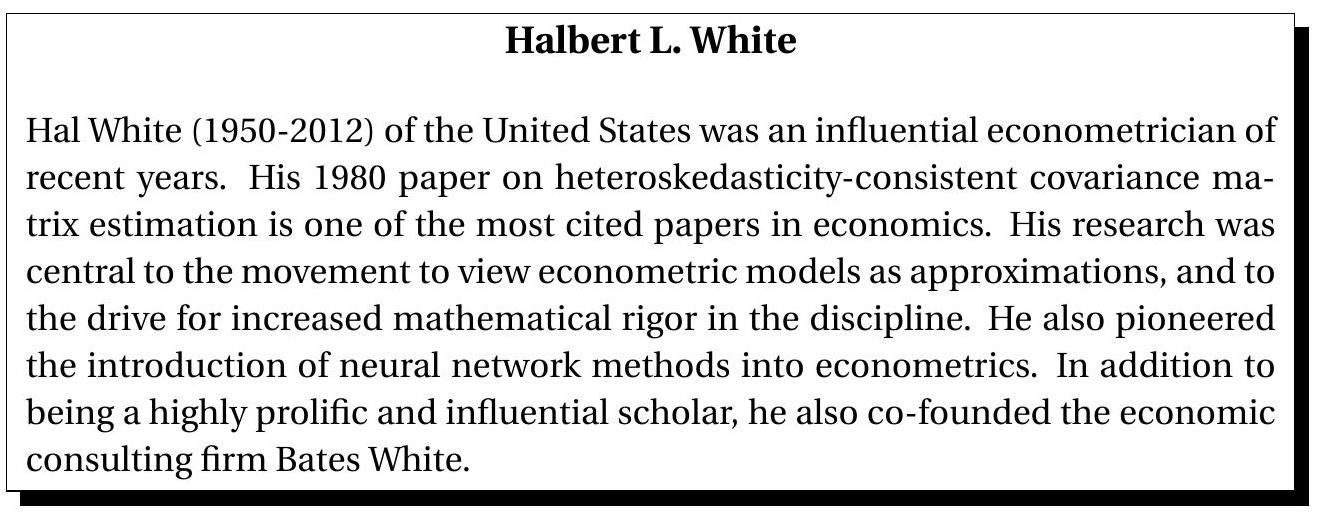
\includegraphics[max width=\textwidth]{2022_09_17_46fafb30295495354ae2g-19}

\subsection{Standard Errors}
A variance estimator such as $\widehat{\boldsymbol{V}}_{\widehat{\beta}}$ is an estimator of the variance of the distribution of $\widehat{\beta}$. A more easily interpretable measure of spread is its square root - the standard deviation. This is so important when discussing the distribution of parameter estimators we have a special name for estimates of their standard deviation.

Definition $4.2$ A standard error $s(\widehat{\beta})$ for a real-valued estimator $\widehat{\beta}$ is an estimator of the standard deviation of the distribution of $\widehat{\beta}$.

When $\beta$ is a vector with estimator $\widehat{\beta}$ and covariance matrix estimator $\widehat{\boldsymbol{V}}_{\widehat{\beta}}$, standard errors for individual elements are the square roots of the diagonal elements of $\widehat{\boldsymbol{V}}_{\widehat{\beta}}$. That is,
$$
s\left(\widehat{\beta}_{j}\right)=\sqrt{\widehat{\boldsymbol{V}}_{\widehat{\beta}_{j}}}=\sqrt{\left[\widehat{\boldsymbol{V}}_{\widehat{\beta}}\right]_{j j}}
$$
When the classical covariance matrix estimator (4.35) is used the standard error takes the simple form
$$
s\left(\widehat{\beta}_{j}\right)=s \sqrt{\left[\left(\boldsymbol{X}^{\prime} \boldsymbol{X}\right)^{-1}\right]_{j j}} .
$$
As we discussed in the previous section there are multiple possible covariance matrix estimators so standard errors are not unique. It is therefore important to understand what formula and method is used by an author when studying their work. It is also important to understand that a particular standard error may be relevant under one set of model assumptions but not under another set of assumptions.

To illustrate, we return to the log wage regression (3.12) of Section 3.7. We calculate that $s^{2}=0.160$. Therefore the homoskedastic covariance matrix estimate is
$$
\widehat{\boldsymbol{V}}_{\widehat{\beta}}^{0}=\left(\begin{array}{cc}
5010 & 314 \\
314 & 20
\end{array}\right)^{-1} 0.160=\left(\begin{array}{cc}
0.002 & -0.031 \\
-0.031 & 0.499
\end{array}\right)
$$
We also calculate that
$$
\sum_{i=1}^{n}\left(1-h_{i i}\right)^{-1} X_{i} X_{i}^{\prime} \widehat{e}_{i}^{2}=\left(\begin{array}{cc}
763.26 & 48.513 \\
48.513 & 3.1078
\end{array}\right) .
$$
Therefore the HC2 covariance matrix estimate is
$$
\begin{aligned}
\widehat{\boldsymbol{V}}_{\widehat{\beta}}^{\mathrm{HC} 2} &=\left(\begin{array}{cc}
5010 & 314 \\
314 & 20
\end{array}\right)^{-1}\left(\begin{array}{cc}
763.26 & 48.513 \\
48.513 & 3.1078
\end{array}\right)\left(\begin{array}{cc}
5010 & 314 \\
314 & 20
\end{array}\right)^{-1} \\
&=\left(\begin{array}{cc}
0.001 & -0.015 \\
-0.015 & 0.243
\end{array}\right) .
\end{aligned}
$$
The standard errors are the square roots of the diagonal elements of these matrices. A conventional format to write the estimated equation with standard errors is

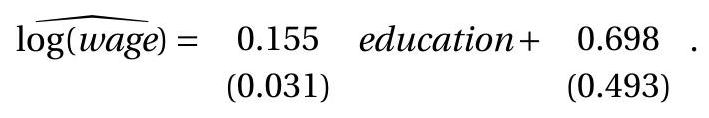
\includegraphics[max width=\textwidth]{2022_09_17_46fafb30295495354ae2g-20}

Alternatively, standard errors could be calculated using the other formulae. We report the different standard errors in the following table.

Table 4.1: Standard Errors

\begin{tabular}{lcc}
\hline\hline
 & Education & Intercept \\
\cline { 2 - 3 }
Homoskedastic (4.35) & $0.045$ & $0.707$ \\
HC0 (4.36) & $0.029$ & $0.461$ \\
HC1 $(4.37)$ & $0.030$ & $0.486$ \\
HC2 $(4.38)$ & $0.031$ & $0.493$ \\
HC3 $(4.39)$ & $0.033$ & $0.527$ \\
\hline
\end{tabular}

The homoskedastic standard errors are noticeably different (larger in this case) than the others. The robust standard errors are reasonably close to one another though the HC3 standard errors are larger than the others.

\subsection{Estimation with Sparse Dummy Variables}
The heteroskedasticity-robust covariance matrix estimators can be quite imprecise in some contexts. One is in the presence of sparse dummy variables - when a dummy variable only takes the value 1 or 0 for very few observations. In these contexts one component of the covariance matrix is estimated on just those few observations and will be imprecise. This is effectively hidden from the user. To see the problem, let $D$ be a dummy variable (takes on the values 1 and 0 ) and consider the dummy variable regression
$$
Y=\beta_{1} D+\beta_{2}+e .
$$
The number of observations for which $D_{i}=1$ is $n_{1}=\sum_{i=1}^{n} D_{i}$. The number of observations for which $D_{i}=0$ is $n_{2}=n-n_{1}$. We say the design is sparse if $n_{1}$ or $n_{2}$ is small.

To simplify our analysis, we take the extreme case $n_{1}=1$. The ideas extend to the case of $n_{1}>1$ but small, though with less dramatic effects.

In the regression model (4.45) we can calculate that the true covariance matrix of the least squares estimator for the coefficients under the simplifying assumption of conditional homoskedasticity is
$$
\boldsymbol{V}_{\widehat{\beta}}=\sigma^{2}\left(\boldsymbol{X}^{\prime} \boldsymbol{X}\right)^{-1}=\sigma^{2}\left(\begin{array}{ll}
1 & 1 \\
1 & n
\end{array}\right)^{-1}=\frac{\sigma^{2}}{n-1}\left(\begin{array}{cc}
n & -1 \\
-1 & 1
\end{array}\right)
$$
In particular, the variance of the estimator for the coefficient on the dummy variable is
$$
V_{\widehat{\beta}_{1}}=\sigma^{2} \frac{n}{n-1} .
$$
Essentially, the coefficient $\beta_{1}$ is estimated from a single observation so its variance is roughly unaffected by sample size. An important message is that certain coefficient estimators in the presence of sparse dummy variables will be imprecise, regardless of the sample size. A large sample alone is not sufficient to ensure precise estimation.

Now let's examine the standard HC1 covariance matrix estimator (4.37). The regression has perfect fit for the observation for which $D_{i}=1$ so the corresponding residual is $\widehat{e}_{i}=0$. It follows that $D_{i} \widehat{e}_{i}=0$ for all $i$ (either $D_{i}=0$ or $\widehat{e}_{i}=0$ ). Hence
$$
\sum_{i=1}^{n} X_{i} X_{i}^{\prime} \hat{e}_{i}^{2}=\left(\begin{array}{cc}
0 & 0 \\
0 & \sum_{i=1}^{n} \widehat{e}_{i}^{2}
\end{array}\right)=\left(\begin{array}{cc}
0 & 0 \\
0 & (n-2) s^{2}
\end{array}\right)
$$
where $s^{2}=(n-2)^{-1} \sum_{i=1}^{n} \widehat{e}_{i}^{2}$ is the bias-corrected estimator of $\sigma^{2}$. Together we find that
$$
\begin{aligned}
\widehat{\boldsymbol{V}}_{\widehat{\beta}}^{\mathrm{HC1}} &=\left(\frac{n}{n-2}\right) \frac{1}{(n-1)^{2}}\left(\begin{array}{cc}
n & -1 \\
-1 & 1
\end{array}\right)\left(\begin{array}{cc}
0 & 0 \\
0 & (n-2) s^{2}
\end{array}\right)\left(\begin{array}{cc}
n & -1 \\
-1 & 1
\end{array}\right) \\
&=s^{2} \frac{n}{(n-1)^{2}}\left(\begin{array}{cc}
1 & -1 \\
-1 & 1
\end{array}\right) .
\end{aligned}
$$
In particular, the estimator for $V_{\widehat{\beta}_{1}}$ is
$$
\widehat{V}_{\widehat{\beta}_{1}}^{\mathrm{HC} 1}=s^{2} \frac{n}{(n-1)^{2}}
$$
It has expectation
$$
\mathbb{E}\left[\widehat{V}_{\widehat{\beta}_{1}}^{\mathrm{HC1}}\right]=\sigma^{2} \frac{n}{(n-1)^{2}}=\frac{V_{\widehat{\beta}_{1}}}{n-1}<<V_{\widehat{\beta}_{1}} .
$$
The variance estimator $\widehat{V}_{\widehat{\beta}_{1}}^{\mathrm{HCl}}$ is extremely biased for $V_{\widehat{\beta}_{1}}$. It is too small by a multiple of $n$ ! The reported variance - and standard error - is misleadingly small. The variance estimate erroneously mis-states the precision of $\widehat{\beta}_{1}$.

The fact that $\widehat{V}_{\widehat{\beta}_{1}}^{\mathrm{HCl}}$ is biased is unlikely to be noticed by an applied researcher. Nothing in the reported output will alert a researcher to the problem. Another way to see the issue is to consider the estimator $\widehat{\theta}=\widehat{\beta}_{1}+\widehat{\beta}_{2}$ for the sum of the coefficients $\theta=\beta_{1}+\beta_{2}$. This estimator has true variance $\sigma^{2}$. The variance estimator, however is $\widehat{\boldsymbol{V}}_{\widehat{\theta}}^{\mathrm{HC1}}=0$ ! (It equals the sum of the four elements in $\widehat{\boldsymbol{V}}_{\widehat{\beta}}^{\mathrm{HC1}}$ ). Clearly, the estimator " 0 " is biased for the true value $\sigma^{2}$.

Another insight is to examine the leverage values. The (single) observation with $D_{i}=1$ has
$$
h_{i i}=\frac{1}{n-1}\left(\begin{array}{ll}
1 & 1
\end{array}\right)\left(\begin{array}{cc}
n & -1 \\
-1 & 1
\end{array}\right)\left(\begin{array}{l}
1 \\
1
\end{array}\right)=1 .
$$
This is an extreme leverage value.

A possible solution is to replace the biased covariance matrix estimator $\widehat{V}_{\widehat{\beta}_{1}}^{\mathrm{HC1}}$ with the unbiased estimator $\widehat{V}_{\widehat{\beta}_{1}}^{\mathrm{HC} 2}$ (unbiased under homoskedasticity) or the conservative estimator $\widehat{V}_{\widehat{\beta}_{1}}^{\mathrm{HC}} .$ Neither approach can be done in the extreme sparse case $n_{1}=1$ (for $\widehat{V}_{\widehat{\beta}_{1}}^{\mathrm{HC} 2}$ and $\widehat{V}_{\widehat{\beta}_{1}}^{\mathrm{HC}}$ cannot be calculated if $h_{i i}=1$ for any observation) but applies otherwise. When $h_{i i}=1$ for an observation then $\widehat{V}_{\widehat{\beta}_{1}}^{\mathrm{HC} 2}$ and $\widehat{V}_{\widehat{\beta}_{1}}^{\mathrm{HC} 3}$ cannot be calculated. In this case unbiased covariance matrix estimation appears to be impossible.

It is unclear if there is a best practice to avoid this situation. Once possibility is to calculate the maximum leverage value. If it is very large calculate the standard errors using several methods to see if variation occurs.

\subsection{Computation}
We illustrate methods to compute standard errors for equation (3.13) extending the code of Section $3.25 .$

\section{Stata do File (continued)}
\begin{itemize}
  \item Homoskedastic formula (4.35):
\end{itemize}
reg wage education experience exp2 if $(\mathrm{mnwf}==1)$

\begin{itemize}
  \item $\quad$ HC1 formula (4.37):
\end{itemize}
reg wage education experience exp2 if $(\operatorname{mnwf}==1), \mathrm{r}$

\begin{itemize}
  \item $\mathrm{HC} 2$ formula (4.38):
\end{itemize}
reg wage education experience $\exp 2$ if $(\mathrm{mnwf}==1)$, vce $(\mathrm{hc} 2)$

\begin{itemize}
  \item $\quad$ HC3 formula (4.39):
\end{itemize}
reg wage education experience exp2 if (mnwf $==1)$, vce $(\mathrm{hc} 3)$

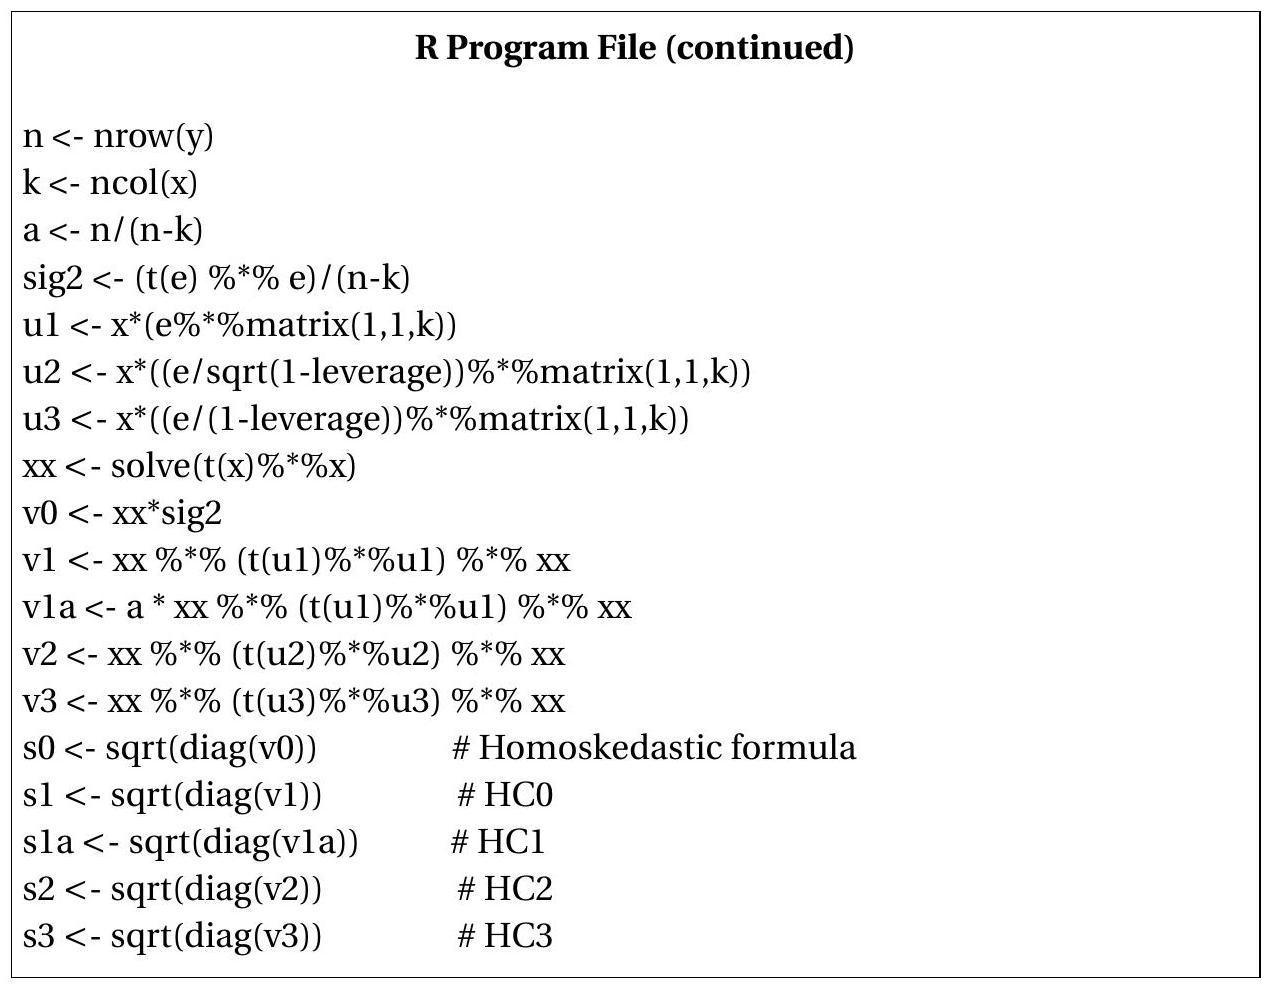
\includegraphics[max width=\textwidth]{2022_09_17_46fafb30295495354ae2g-23}

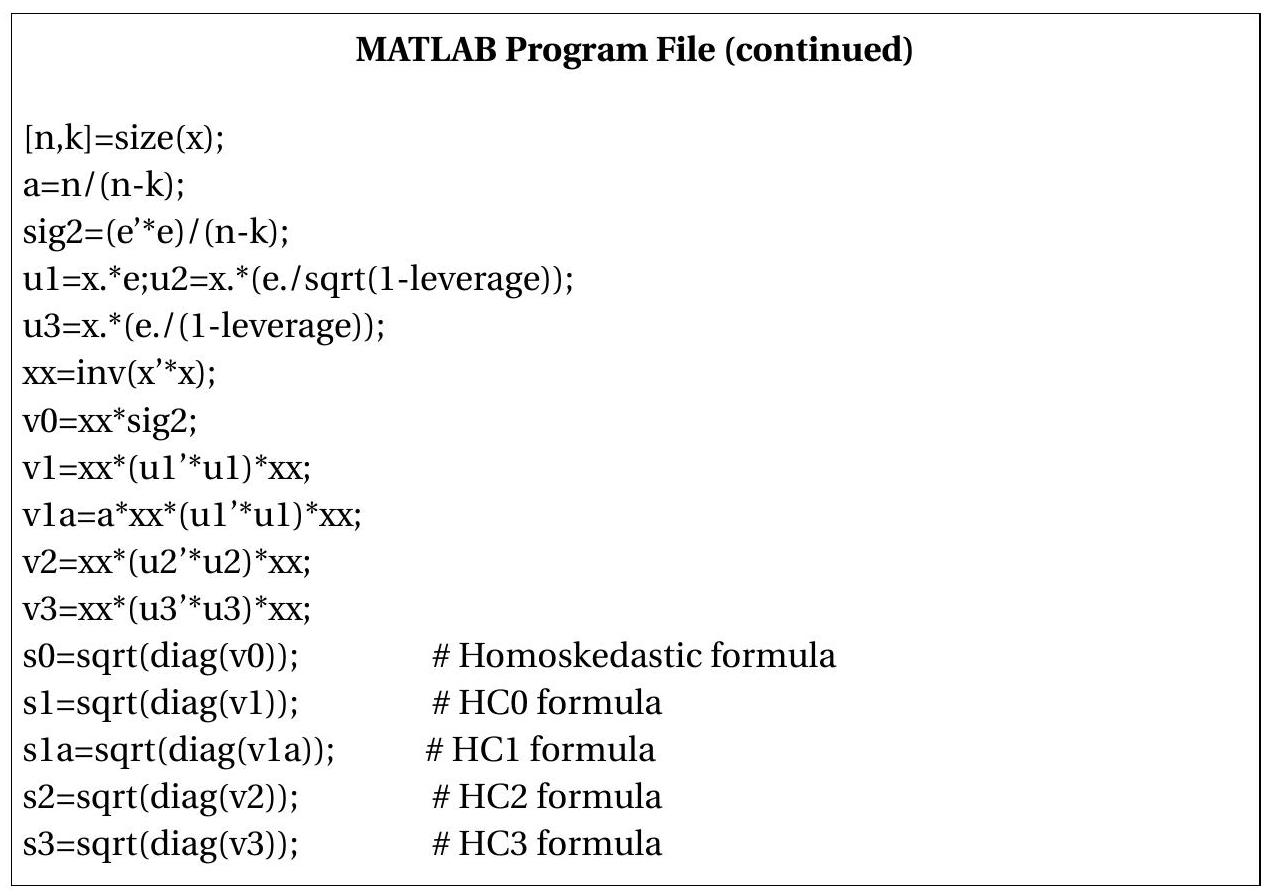
\includegraphics[max width=\textwidth]{2022_09_17_46fafb30295495354ae2g-23(1)}

\subsection{Measures of Fit}
As we described in the previous chapter a commonly reported measure of regression fit is the regression $R^{2}$ defined as
$$
R^{2}=1-\frac{\sum_{i=1}^{n} \widehat{e}_{i}^{2}}{\sum_{i=1}^{n}\left(Y_{i}-\bar{Y}\right)^{2}}=1-\frac{\widehat{\sigma}^{2}}{\widehat{\sigma}_{Y}^{2}} .
$$
where $\widehat{\sigma}_{Y}^{2}=n^{-1} \sum_{i=1}^{n}\left(Y_{i}-\bar{Y}\right)^{2} \cdot R^{2}$ is an estimator of the population parameter
$$
\rho^{2}=\frac{\operatorname{var}\left[X^{\prime} \beta\right]}{\operatorname{var}[Y]}=1-\frac{\sigma^{2}}{\sigma_{Y}^{2}} .
$$
However, $\widehat{\sigma}^{2}$ and $\widehat{\sigma}_{Y}^{2}$ are biased. Theil (1961) proposed replacing these by the unbiased versions $s^{2}$ and $\widetilde{\sigma}_{Y}^{2}=(n-1)^{-1} \sum_{i=1}^{n}\left(Y_{i}-\bar{Y}\right)^{2}$ yielding what is known as R-bar-squared or adjusted R-squared:
$$
\bar{R}^{2}=1-\frac{s^{2}}{\widetilde{\sigma}_{Y}^{2}}=1-\frac{(n-1)^{-1} \sum_{i=1}^{n} \widehat{e}_{i}^{2}}{(n-k)^{-1} \sum_{i=1}^{n}\left(Y_{i}-\bar{Y}\right)^{2}} .
$$
While $\bar{R}^{2}$ is an improvement on $R^{2}$ a much better improvement is
$$
\widetilde{R}^{2}=1-\frac{\sum_{i=1}^{n} \widetilde{e}_{i}^{2}}{\sum_{i=1}^{n}\left(Y_{i}-\bar{Y}\right)^{2}}=1-\frac{\widetilde{\sigma}^{2}}{\widehat{\sigma}_{Y}^{2}}
$$
where $\widetilde{e}_{i}$ are the prediction errors (3.44) and $\widetilde{\sigma}^{2}$ is the MSPE from (3.46). As described in Section (4.12) $\widetilde{\sigma}^{2}$ is a good estimator of the out-of-sample mean-squared forecast error so $\widetilde{R}^{2}$ is a good estimator of the percentage of the forecast variance which is explained by the regression forecast. In this sense $\widetilde{R}^{2}$ is a good measure of fit.

One problem with $R^{2}$ which is partially corrected by $\bar{R}^{2}$ and fully corrected by $\widetilde{R}^{2}$ is that $R^{2}$ necessarily increases when regressors are added to a regression model. This occurs because $R^{2}$ is a negative function of the sum of squared residuals which cannot increase when a regressor is added. In contrast, $\bar{R}^{2}$ and $\widetilde{R}^{2}$ are non-monotonic in the number of regressors. $\widetilde{R}^{2}$ can even be negative, which occurs when an estimated model predicts worse than a constant-only model.

In the statistical literature the MSPE $\widetilde{\sigma}^{2}$ is known as the leave-one-out cross validation criterion and is popular for model comparison and selection, especially in high-dimensional and nonparametric contexts. It is equivalent to use $\widetilde{R}^{2}$ or $\widetilde{\sigma}^{2}$ to compare and select models. Models with high $\widetilde{R}^{2}$ (or low $\widetilde{\sigma}^{2}$ ) are better models in terms of expected out of sample squared error. In contrast, $R^{2}$ cannot be used for model selection as it necessarily increases when regressors are added to a regression model. $\bar{R}^{2}$ is also an inappropriate choice for model selection (it tends to select models with too many parameters) though a justification of this assertion requires a study of the theory of model selection. Unfortunately, $\bar{R}^{2}$ is routinely used by some economists, possibly as a hold-over from previous generations.

In summary, it is recommended to omit $R^{2}$ and $\bar{R}^{2}$. If a measure of fit is desired, report $\widetilde{R}^{2}$ or $\widetilde{\sigma}^{2}$.

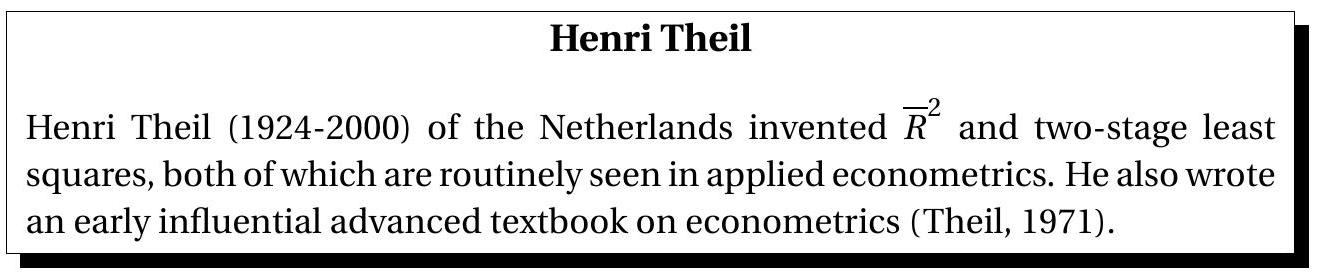
\includegraphics[max width=\textwidth]{2022_09_17_46fafb30295495354ae2g-24}

\subsection{Empirical Example}
We again return to our wage equation but use a much larger sample of all individuals with at least 12 years of education. For regressors we include years of education, potential work experience, experience squared, and dummy variable indicators for the following: female, female union member, male union member, married female ${ }^{1}$, married male, formerly married female ${ }^{2}$, formerly married male, Hispanic, Black, American Indian, Asian, and mixed race ${ }^{3}$. The available sample is 46,943 so the parameter estimates are quite precise and reported in Table 4.2. For standard errors we use the unbiased HC2 formula.

Table $4.2$ displays the parameter estimates in a standard tabular format. Parameter estimates and standard errors are reported for all coefficients. In addition to the coefficient estimates the table also reports the estimated error standard deviation and the sample size. These are useful summary measures of fit which aid readers.

Table 4.2: OLS Estimates of Linear Equation for $\log ($ wage $)$

\begin{tabular}{lrr}
\hline\hline
 &  &  \\
 & $\widehat{\beta}$ & $s(\widehat{\beta})$ \\
\cline { 2 - 3 }
Education & $0.117$ & $0.001$ \\
Experience & $0.033$ & $0.001$ \\
Experience $^{2} / 100$ & $-0.056$ & $0.002$ \\
Female & $-0.098$ & $0.011$ \\
Female Union Member & $0.023$ & $0.020$ \\
Male Union Member & $0.095$ & $0.020$ \\
Married Female & $0.016$ & $0.010$ \\
Married Male & $0.211$ & $0.010$ \\
Formerly Married Female & $-0.006$ & $0.012$ \\
Formerly Married Male & $0.083$ & $0.015$ \\
Hispanic & $-0.108$ & $0.008$ \\
Black & $-0.096$ & $0.008$ \\
American Indian & $-0.137$ & $0.027$ \\
Asian & $-0.038$ & $0.013$ \\
Mixed Race & $-0.041$ & $0.021$ \\
Intercept & $0.909$ & $0.021$ \\
$\widehat{\sigma}$ & $0.565$ &  \\
Sample Size & 46,943 &  \\
\hline
\end{tabular}

Standard errors are heteroskedasticity-consistent (Horn-Horn-Duncan formula).

As a general rule it is advisable to always report standard errors along with parameter estimates. This allows readers to assess the precision of the parameter estimates, and as we will discuss in later chapters, form confidence intervals and t-tests for individual coefficients if desired.

The results in Table $4.2$ confirm our earlier findings that the return to a year of education is approximately $12 \%$, the return to experience is concave, single women earn approximately $10 \%$ less then single men, and Blacks earn about $10 \%$ less than whites. In addition, we see that Hispanics earn about $11 \%$ less than whites, American Indians $14 \%$ less, and Asians and Mixed races about $4 \%$ less. We also see there

${ }^{1}$ Defining "married" as marital code 1,2 , or $3 .$

${ }^{2}$ Defining "formerly married" as marital code 4,5 , or 6 .

${ }^{3}$ Race code 6 or higher. are wage premiums for men who are members of a labor union (about $10 \%$ ), married (about 21\%) or formerly married (about $8 \%$ ), but no similar premiums are apparent for women.

\subsection{Multicollinearity}
As discussed in Section 3.24, if $\boldsymbol{X}^{\prime} \boldsymbol{X}$ is singular then $\left(\boldsymbol{X}^{\prime} \boldsymbol{X}\right)^{-1}$ and $\widehat{\beta}$ are not defined. This situation is called strict multicollinearity as the columns of $\boldsymbol{X}$ are linearly dependent, i.e., there is some $\alpha \neq 0$ such that $\boldsymbol{X} \alpha=0$. Most commonly this arises when sets of regressors are included which are identically related. In Section $3.24$ we discussed possible causes of strict multicollinearity and discussed the related problem of ill-conditioning which can cause numerical inaccuracies in severe cases.

A related common situation is near multicollinearity which is often called "multicollinearity" for brevity. This is the situation when the regressors are highly correlated. An implication of near multicollinearity is that individual coefficient estimates will be imprecise. This is not necessarily a problem for econometric analysis if the reported standard errors are accurate. However, robust standard errors can be sensitive to large leverage values which can occur under near multicollinearity. This leads to the undesirable situation where the coefficient estimates are imprecise yet the standard errors are misleadingly small.

We can see the impact of near multicollinearity on precision in a simple homoskedastic linear regression model with two regressors
$$
Y=X_{1} \beta_{1}+X_{2} \beta_{2}+e
$$
and
$$
\frac{1}{n} \boldsymbol{X}^{\prime} \boldsymbol{X}=\left(\begin{array}{ll}
1 & \rho \\
\rho & 1
\end{array}\right) .
$$
In this case
$$
\operatorname{var}[\widehat{\beta} \mid \boldsymbol{X}]=\frac{\sigma^{2}}{n}\left(\begin{array}{ll}
1 & \rho \\
\rho & 1
\end{array}\right)^{-1}=\frac{\sigma^{2}}{n\left(1-\rho^{2}\right)}\left(\begin{array}{cc}
1 & -\rho \\
-\rho & 1
\end{array}\right) .
$$
The correlation $\rho$ indexes collinearity since as $\rho$ approaches 1 the matrix becomes singular. We can see the effect of collinearity on precision by observing that the variance of a coefficient estimate $\sigma^{2}\left[n\left(1-\rho^{2}\right)\right]^{-1}$ approaches infinity as $\rho$ approaches 1 . Thus the more "collinear" are the regressors the worse the precision of the individual coefficient estimates.

What is happening is that when the regressors are highly dependent it is statistically difficult to disentangle the impact of $\beta_{1}$ from that of $\beta_{2}$. As a consequence the precision of individual estimates are reduced.

Many early-generation textbooks overemphasized multicollinearity. An amusing parody of these texts is Micronumerosity, Chapter $23.3$ of Goldberger's A Course in Econometrics (1991). Among the witty remarks of his chapter are the following.

The extreme case, 'exact micronumerosity', arises when $n=0$, in which case the sample estimate of $\mu$ is not unique. (Technically, there is a violation of the rank condition $n>0$ : the matrix 0 is singular.)

Tests for the presence of micronumerosity require the judicious use of various fingers. Some researchers prefer a single finger, others use their toes, still others let their thumbs rule.

A generally reliable guide may be obtained by counting the number of observations. Most of the time in econometric analysis, when $n$ is close to zero, it is also far from infinity.

Arthur S. Goldberger, A Course in Econometrics (1991), pp. $249 .$ To understand Goldberger's basic point you should notice that the estimation variance $\sigma^{2}\left[n\left(1-\rho^{2}\right)\right]^{-1}$ depends equally and symmetrically on the correlation $\rho$ and the sample size $n$. He was pointing out that the only statistical implication of multicollinearity in the homoskedastic model is a lack of precision. Small sample sizes have the exact same implication.

\begin{tabular}{|l|}
\hline
\multicolumn{1}{c|}{Arthur S. Goldberger} \\
Art Goldberger (1930-2009) was one of the most distinguished members of the \\
Department of Economics at the University of Wisconsin. His Ph.D. thesis devel- \\
oped a pioneering macroeconometric forecasting model (the Klein-Goldberger \\
model). Most of his remaining career focused on microeconometric issues. He \\
was the leading pioneer of what has been called the Wisconsin Tradition of em- \\
pirical work - a combination of formal econometric theory with a careful critical \\
analysis of empirical work. Goldberger wrote a series of highly regarded and in- \\
fluential graduate econometric textbooks, including Econometric Theory (1964), \\
Topics in Regression Analysis (1968), and A Course in Econometrics (1991). \\
\end{tabular}

\subsection{Clustered Sampling}
In Section $4.2$ we briefly mentioned clustered sampling as an alternative to the assumption of random sampling. We now introduce the framework in more detail and extend the primary results of this chapter to encompass clustered dependence.

It might be easiest to understand the idea of clusters by considering a concrete example. Duflo, Dupas, and Kremer (2011) investigate the impact of tracking (assigning students based on initial test score) on educational attainment in a randomized experiment. An extract of their data set is available on the textbook webpage in the file DDK2011.

In 2005, 140 primary schools in Kenya received funding to hire an extra first grade teacher to reduce class sizes. In half of the schools (selected randomly) students were assigned to classrooms based on an initial test score ("tracking"); in the remaining schools the students were randomly assigned to classrooms. For their analysis the authors restricted attention to the 121 schools which initially had a single first-grade class.

The key regression ${ }^{4}$ in the paper is
$$
\text { TestScore }_{i g}=-0.071+0.138 \text { Tracking }_{g}+e_{i g}
$$
where TestScore ${ }_{i g}$ is the standardized test score (normalized to have mean 0 and variance 1) of student $i$ in school $g$, and Tracking $g$ is a dummy equal to 1 if school $g$ was tracking. The OLS estimates indicate that schools which tracked the students had an overall increase in test scores by about $0.14$ standard deviations, which is meaningful. More general versions of this regression are estimated, many of which take the form
$$
\text { TestScore }_{i g}=\alpha+\gamma \text { Tracking }_{g}+X_{i g}^{\prime} \beta+e_{i g}
$$
where $X_{i g}$ is a set of controls specific to the student (including age, gender, and initial test score).

${ }^{4}$ Table 2, column (1). Duflo, Dupas and Kremer (2011) report a coefficient estimate of $0.139$, perhaps due to a slightly different calculation to standardize the test score. A difficulty with applying the classical regression framework is that student achievement is likely correlated within a given school. Student achievement may be affected by local demographics, individual teachers, and classmates, all of which imply dependence. These concerns, however, do not suggest that achievement will be correlated across schools, so it seems reasonable to model achievement across schools as mutually independent. We call such dependence clustered.

In clustering contexts it is convenient to double index the observations as $\left(Y_{i g}, X_{i g}\right)$ where $g=1, \ldots, G$ indexes the cluster and $i=1, \ldots, n_{g}$ indexes the individual within the $g^{t h}$ cluster. The number of observations per cluster $n_{g}$ may vary across clusters. The number of clusters is $G$. The total number of observations is $n=\sum_{g=1}^{G} n_{g}$. In the Kenyan schooling example the number of clusters (schools) in the estimation sample is $G=121$, the number of students per school varies from 19 to 62 , and the total number of observations is $n=5795$.

While it is typical to write the observations using the double index notation $\left(Y_{i g}, X_{i g}\right)$ it is also useful to use cluster-level notation. Let $\boldsymbol{Y}_{g}=\left(Y_{1 g}, \ldots, Y_{n_{g} g}\right)^{\prime}$ and $\boldsymbol{X}_{g}=\left(X_{1 g}, \ldots, X_{n_{g} g}\right)^{\prime}$ denote the $n_{g} \times 1$ vector of dependent variables and $n_{g} \times k$ matrix of regressors for the $g^{t h}$ cluster. A linear regression model can be written by individual as
$$
Y_{i g}=X_{i g}^{\prime} \beta+e_{i g}
$$
and using cluster notation as
$$
\boldsymbol{Y}_{g}=\boldsymbol{X}_{g} \beta+\boldsymbol{e}_{g}
$$
where $\boldsymbol{e}_{g}=\left(e_{1 g}, \ldots, e_{n_{g} g}\right)^{\prime}$ is a $n_{g} \times 1$ error vector. We can also stack the observations into full sample matrices and write the model as
$$
\boldsymbol{Y}=\boldsymbol{X} \beta+\boldsymbol{e} .
$$
Using this notation we can write the sums over the observations using the double sum $\sum_{g=1}^{G} \sum_{i=1}^{n_{g}}$. This is the sum across clusters of the sum across observations within each cluster. The OLS estimator can be written as
$$
\begin{aligned}
\widehat{\beta} &=\left(\sum_{g=1}^{G} \sum_{i=1}^{n_{g}} X_{i g} X_{i g}^{\prime}\right)^{-1}\left(\sum_{g=1}^{G} \sum_{i=1}^{n_{g}} X_{i g} Y_{i g}\right) \\
&=\left(\sum_{g=1}^{G} \boldsymbol{X}_{g}^{\prime} \boldsymbol{X}_{g}\right)^{-1}\left(\sum_{g=1}^{G} \boldsymbol{X}_{g}^{\prime} \boldsymbol{Y}_{g}\right) \\
&=\left(\boldsymbol{X}^{\prime} \boldsymbol{X}\right)^{-1}\left(\boldsymbol{X}^{\prime} \boldsymbol{Y}\right)
\end{aligned}
$$
The residuals are $\widehat{e}_{i g}=Y_{i g}-X_{i g}^{\prime} \widehat{\beta}$ in individual level notation and $\widehat{\boldsymbol{e}}_{g}=\boldsymbol{Y}_{g}-\boldsymbol{X}_{g} \widehat{\beta}$ in cluster level notation.

The standard clustering assumption is that the clusters are known to the researcher and that the observations are independent across clusters.

Assumption 4.4 The clusters $\left(\boldsymbol{Y}_{g}, \boldsymbol{X}_{g}\right)$ are mutually independent across clusters $g$.

In our example clusters are schools. In other common applications cluster dependence has been assumed within individual classrooms, families, villages, regions, and within larger units such as industries and states. This choice is up to the researcher though the justification will depend on the context, the nature of the data, and will reflect information and assumptions on the dependence structure across observations. The model is a linear regression under the assumption
$$
\mathbb{E}\left[\boldsymbol{e}_{g} \mid \boldsymbol{X}_{g}\right]=0 .
$$
This is the same as assuming that the individual errors are conditionally mean zero
$$
\mathbb{E}\left[e_{i g} \mid \boldsymbol{X}_{g}\right]=0
$$
or that the conditional expectation of $\boldsymbol{Y}_{g}$ given $\boldsymbol{X}_{g}$ is linear. As in the independent case equation (4.50) means that the linear regression model is correctly specified. In the clustered regression model this requires that all interaction effects within clusters have been accounted for in the specification of the individual regressors $X_{i g}$.

In the regression (4.46) the conditional expectation is necessarily linear and satisfies (4.50) since the

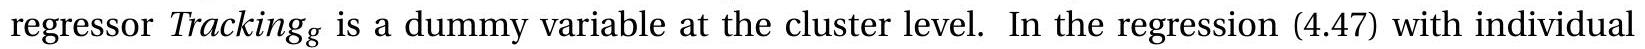
\includegraphics[max width=\textwidth]{2022_09_17_46fafb30295495354ae2g-29}\\
controls, (4.50) requires that the achievement of any student is unaffected by the individual controls (e.g. age, gender, and initial test score) of other students within the same school.

Given (4.50) we can calculate the expectation of the OLS estimator. Substituting (4.48) into (4.49) we find
$$
\widehat{\beta}-\beta=\left(\sum_{g=1}^{G} \boldsymbol{X}_{g}^{\prime} \boldsymbol{X}_{g}\right)^{-1}\left(\sum_{g=1}^{G} \boldsymbol{X}_{g}^{\prime} \boldsymbol{e}_{g}\right)
$$
The mean of $\widehat{\beta}-\beta$ conditioning on all the regressors is
$$
\begin{aligned}
\mathbb{E}[\widehat{\beta}-\beta \mid \boldsymbol{X}] &=\left(\sum_{g=1}^{G} \boldsymbol{X}_{g}^{\prime} \boldsymbol{X}_{g}\right)^{-1}\left(\sum_{g=1}^{G} \boldsymbol{X}_{g}^{\prime} \mathbb{E}\left[\boldsymbol{e}_{g} \mid \boldsymbol{X}\right]\right) \\
&=\left(\sum_{g=1}^{G} \boldsymbol{X}_{g}^{\prime} \boldsymbol{X}_{g}\right)^{-1}\left(\sum_{g=1}^{G} \boldsymbol{X}_{g}^{\prime} \mathbb{E}\left[\boldsymbol{e}_{g} \mid \boldsymbol{X}_{g}\right]\right) \\
&=0 .
\end{aligned}
$$
The first equality holds by linearity, the second by Assumption 4.4, and the third by (4.50).

This shows that OLS is unbiased under clustering if the conditional expectation is linear.

Theorem 4.7 In the clustered linear regression model (Assumption $4.4$ and (4.50)) $\mathbb{E}[\widehat{\beta} \mid \boldsymbol{X}]=\beta$.

Now consider the covariance matrix of $\widehat{\beta}$. Let $\Sigma_{g}=\mathbb{E}\left[\boldsymbol{e}_{g} \boldsymbol{e}_{g}^{\prime} \mid \boldsymbol{X}_{g}\right]$ denote the $n_{g} \times n_{g}$ conditional covariance matrix of the errors within the $g^{t h}$ cluster. Since the observations are independent across clusters,
$$
\begin{aligned}
\operatorname{var}\left[\left(\sum_{g=1}^{G} \boldsymbol{X}_{g}^{\prime} \boldsymbol{e}_{g}\right) \mid \boldsymbol{X}\right] &=\sum_{g=1}^{G} \operatorname{var}\left[\boldsymbol{X}_{g}^{\prime} \boldsymbol{e}_{g} \mid \boldsymbol{X}_{g}\right] \\
&=\sum_{g=1}^{G} \boldsymbol{X}_{g}^{\prime} \mathbb{E}\left[\boldsymbol{e}_{g} \boldsymbol{e}_{g}^{\prime} \mid \boldsymbol{X}_{g}\right] \boldsymbol{X}_{g} \\
&=\sum_{g=1}^{G} \boldsymbol{X}_{g}^{\prime} \Sigma_{g} \boldsymbol{X}_{g} \\
& \stackrel{\text { def }}{=} \Omega_{n}
\end{aligned}
$$
It follows that
$$
\boldsymbol{V}_{\widehat{\beta}}=\operatorname{var}[\widehat{\beta} \mid \boldsymbol{X}]=\left(\boldsymbol{X}^{\prime} \boldsymbol{X}\right)^{-1} \Omega_{n}\left(\boldsymbol{X}^{\prime} \boldsymbol{X}\right)^{-1} .
$$
This differs from the formula in the independent case due to the correlation between observations within clusters. The magnitude of the difference depends on the degree of correlation between observations within clusters and the number of observations within clusters. To see this, suppose that all clusters have the same number of observations $n_{g}=N, \mathbb{E}\left[e_{i g}^{2} \mid \boldsymbol{X}_{g}\right]=\sigma^{2}, \mathbb{E}\left[e_{i g} e_{\ell g} \mid \boldsymbol{X}_{g}\right]=\sigma^{2} \rho$ for $i \neq \ell$, and the regressors $X_{i g}$ do not vary within a cluster. In this case the exact variance of the OLS estimator equals ${ }^{5}$ (after some calculations)
$$
\boldsymbol{V}_{\widehat{\beta}}=\left(\boldsymbol{X}^{\prime} \boldsymbol{X}\right)^{-1} \sigma^{2}(1+\rho(N-1)) .
$$
If $\rho>0$ the exact variance is appropriately a multiple $\rho N$ of the conventional formula. In the Kenyan school example the average cluster size is 48 . If $\rho=0.25$ this means the exact variance exceeds the conventional formula by a factor of about twelve. In this case the correct standard errors (the square root of the variance) are a multiple of about three times the conventional formula. This is a substantial difference and should not be neglected.

Arellano (1987) proposed a cluster-robust covariance matrix estimator which is an extension of the White estimator. Recall that the insight of the White covariance estimator is that the squared error $e_{i}^{2}$ is unbiased for $\mathbb{E}\left[e_{i}^{2} \mid X_{i}\right]=\sigma_{i}^{2}$. Similarly, with cluster dependence the matrix $\boldsymbol{e}_{g} \boldsymbol{e}_{g}^{\prime}$ is unbiased for $\mathbb{E}\left[\boldsymbol{e}_{g} \boldsymbol{e}_{g}^{\prime} \mid \boldsymbol{X}_{g}\right]=\Sigma_{g}$. This means that an unbiased estimator for (4.51) is $\widetilde{\Omega}_{n}=\sum_{g=1}^{G} \boldsymbol{X}_{g}^{\prime} \boldsymbol{e}_{g} \boldsymbol{e}_{g}^{\prime} \boldsymbol{X}_{g}$. This is not feasible, but we can replace the unknown errors by the OLS residuals to obtain Arellano's estimator:
$$
\begin{aligned}
\widehat{\Omega}_{n} &=\sum_{g=1}^{G} \boldsymbol{X}_{g}^{\prime} \widehat{\boldsymbol{e}}_{g} \widehat{\boldsymbol{e}}_{g}^{\prime} \boldsymbol{X}_{g} \\
&=\sum_{g=1}^{G} \sum_{i=1}^{n_{g}} \sum_{\ell=1}^{n_{g}} X_{i g} X_{\ell g}^{\prime} \widehat{e}_{i g} \widehat{e}_{\ell g} \\
&=\sum_{g=1}^{G}\left(\sum_{i=1}^{n_{g}} X_{i g} \widehat{e}_{i g}\right)\left(\sum_{\ell=1}^{n_{g}} X_{\ell g} \widehat{e}_{\ell g}\right)^{\prime} .
\end{aligned}
$$
The three expressions in (4.54) give three equivalent formulae which could be used to calculate $\widehat{\Omega}_{n}$. The final expression writes $\widehat{\Omega}_{n}$ in terms of the cluster sums $\sum_{\ell=1}^{n_{g}} X_{\ell g} \widehat{e}_{\ell g}$ which is the basis for our example $\mathrm{R}$ and MATLAB codes shown below.

Given the expressions (4.51)-(4.52) a natural cluster covariance matrix estimator takes the form
$$
\widehat{\boldsymbol{V}}_{\widehat{\beta}}=a_{n}\left(\boldsymbol{X}^{\prime} \boldsymbol{X}\right)^{-1} \widehat{\Omega}_{n}\left(\boldsymbol{X}^{\prime} \boldsymbol{X}\right)^{-1}
$$
where $a_{n}$ is a possible finite-sample adjustment. The Stata cluster command uses
$$
a_{n}=\left(\frac{n-1}{n-k}\right)\left(\frac{G}{G-1}\right) .
$$
The factor $G /(G-1)$ was derived by Chris Hansen (2007) in the context of equal-sized clusters to improve performance when the number of clusters $G$ is small. The factor $(n-1) /(n-k)$ is an $a d$ hoc generalization which nests the adjustment used in (4.37) since $G=n$ implies the simplification $a_{n}=n /(n-k)$.

Alternative cluster-robust covariance matrix estimators can be constructed using cluster-level prediction errors such as $\widetilde{\boldsymbol{e}}_{g}=\boldsymbol{Y}_{g}-\boldsymbol{X}_{g} \widehat{\beta}_{(-g)}$ where $\widehat{\beta}_{(-g)}$ is the least squares estimator omitting cluster $g$. As in Section 3.20, we can show that
$$
\widetilde{\boldsymbol{e}}_{g}=\left(\boldsymbol{I}_{n_{g}}-\boldsymbol{X}_{g}\left(\boldsymbol{X}^{\prime} \boldsymbol{X}\right)^{-1} \boldsymbol{X}_{g}^{\prime}\right)^{-1} \widehat{\boldsymbol{e}}_{g}
$$
${ }^{5}$ This formula is due to Moulton (1990). and
$$
\widehat{\beta}_{(-g)}=\widehat{\beta}-\left(\boldsymbol{X}^{\prime} \boldsymbol{X}\right)^{-1} \boldsymbol{X}_{g}^{\prime} \widetilde{\boldsymbol{e}}_{g} .
$$
We then have the robust covariance matrix estimator
$$
\widehat{\boldsymbol{V}}_{\widehat{\beta}}^{\mathrm{CR} 3}=\left(\boldsymbol{X}^{\prime} \boldsymbol{X}\right)^{-1}\left(\sum_{g=1}^{G} \boldsymbol{X}_{g}^{\prime} \widetilde{\boldsymbol{e}}_{g} \widetilde{\boldsymbol{e}}_{g}^{\prime} \boldsymbol{X}_{g}\right)\left(\boldsymbol{X}^{\prime} \boldsymbol{X}\right)^{-1} .
$$
The label "CR" refers to "cluster-robust" and "CR3" refers to the analogous formula for the HC3 estimator.

Similarly to the heteroskedastic-robust case you can show that CR3 is a conservative estimator for $\boldsymbol{V}_{\widehat{\beta}}$ in the sense that the conditional expectation of $\widehat{\boldsymbol{V}}_{\widehat{\beta}}^{\mathrm{CR} 3}$ exceeds $\boldsymbol{V}_{\widehat{\beta}}$. This covariance matrix estimator is more cumbersome to implement, however, as the cluster-level prediction errors (4.57) cannot be calculated in a simple linear operation and requires a loop across clusters to calculate.

To illustrate in the context of the Kenyan schooling example we present the regression of student test scores on the school-level tracking dummy with two standard errors displayed. The first (in parenthesis) is the conventional robust standard error. The second [in square brackets] is the clustered standard error (4.55)-(4.56) where clustering is at the level of the school.

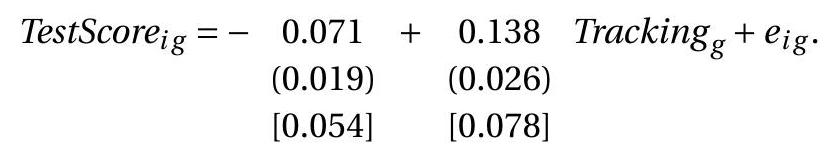
\includegraphics[max width=\textwidth]{2022_09_17_46fafb30295495354ae2g-31}

We can see that the cluster-robust standard errors are roughly three times the conventional robust standard errors. Consequently, confidence intervals for the coefficients are greatly affected by the choice.

For illustration, we list here the commands needed to produce the regression results with clustered standard errors in Stata, R, and MATLAB.

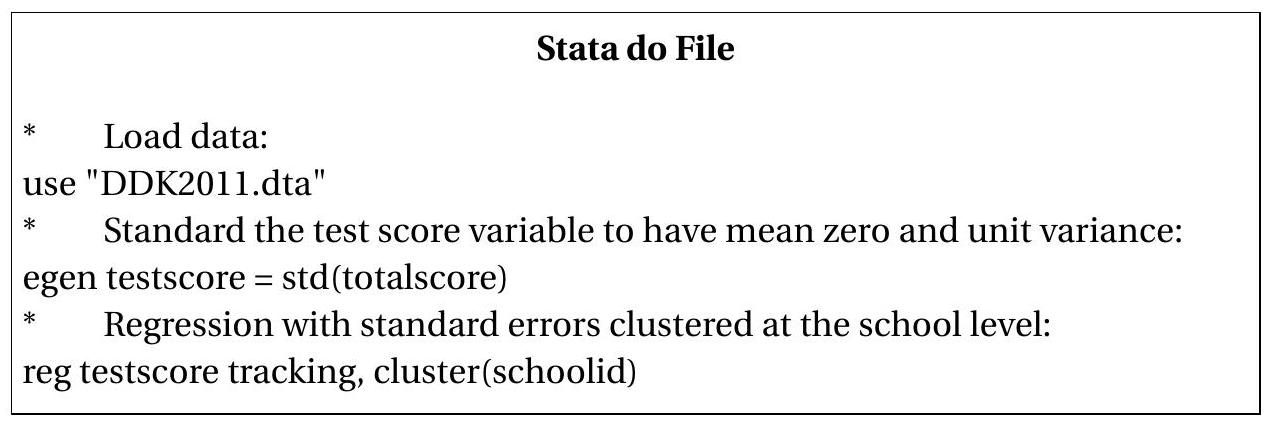
\includegraphics[max width=\textwidth]{2022_09_17_46fafb30295495354ae2g-31(1)}

You can see that clustered standard errors are simple to calculate in Stata.

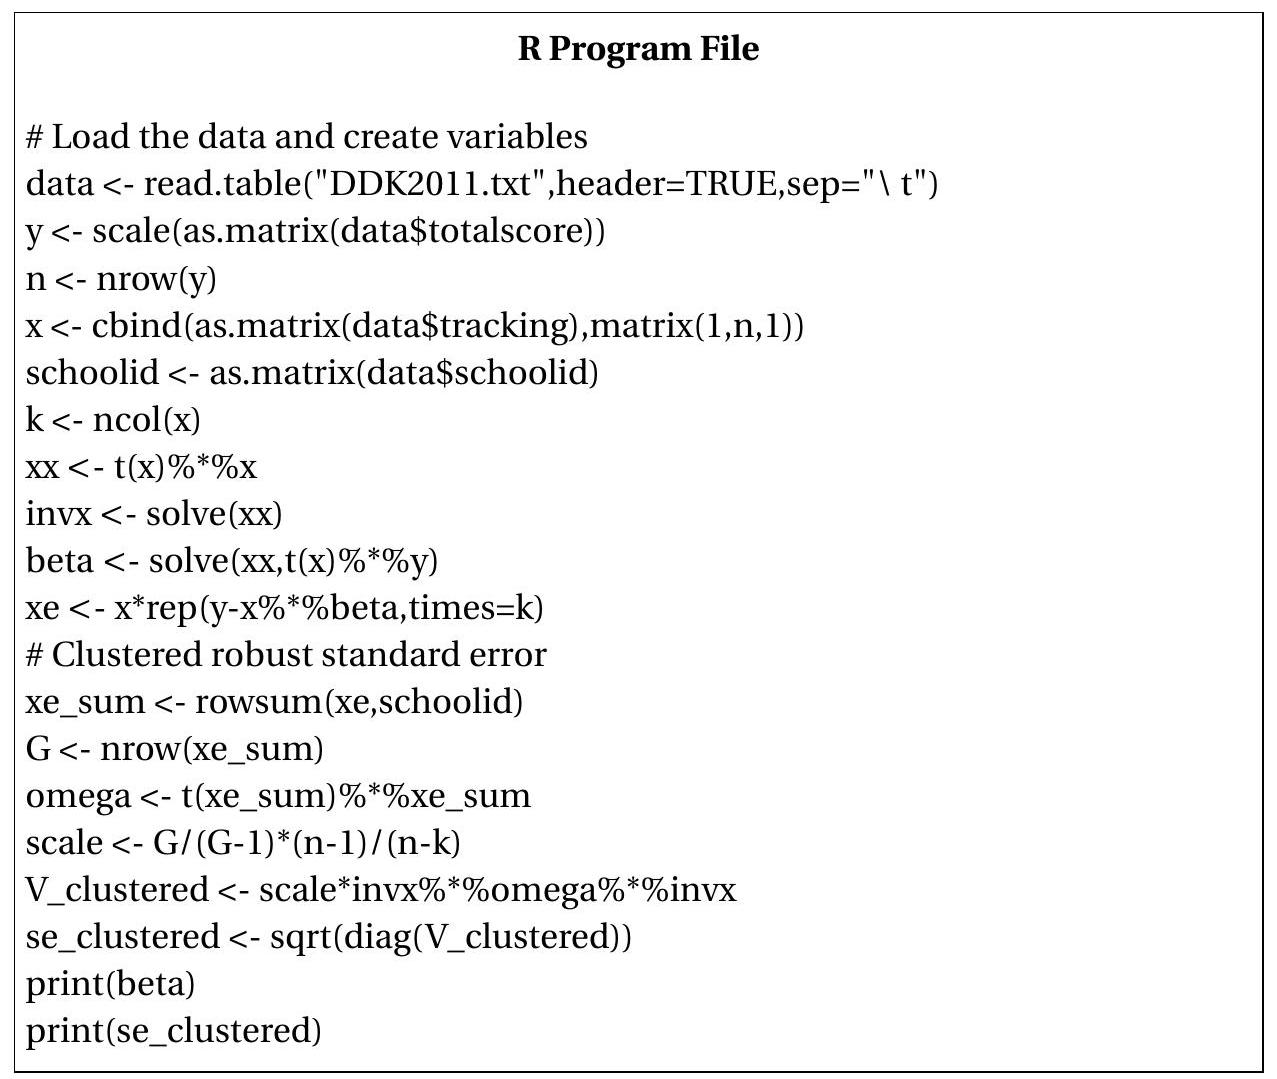
\includegraphics[max width=\textwidth]{2022_09_17_46fafb30295495354ae2g-32}

Programming clustered standard errors in $\mathrm{R}$ is also relatively easy due to the convenient rowsum command which sums variables within clusters.

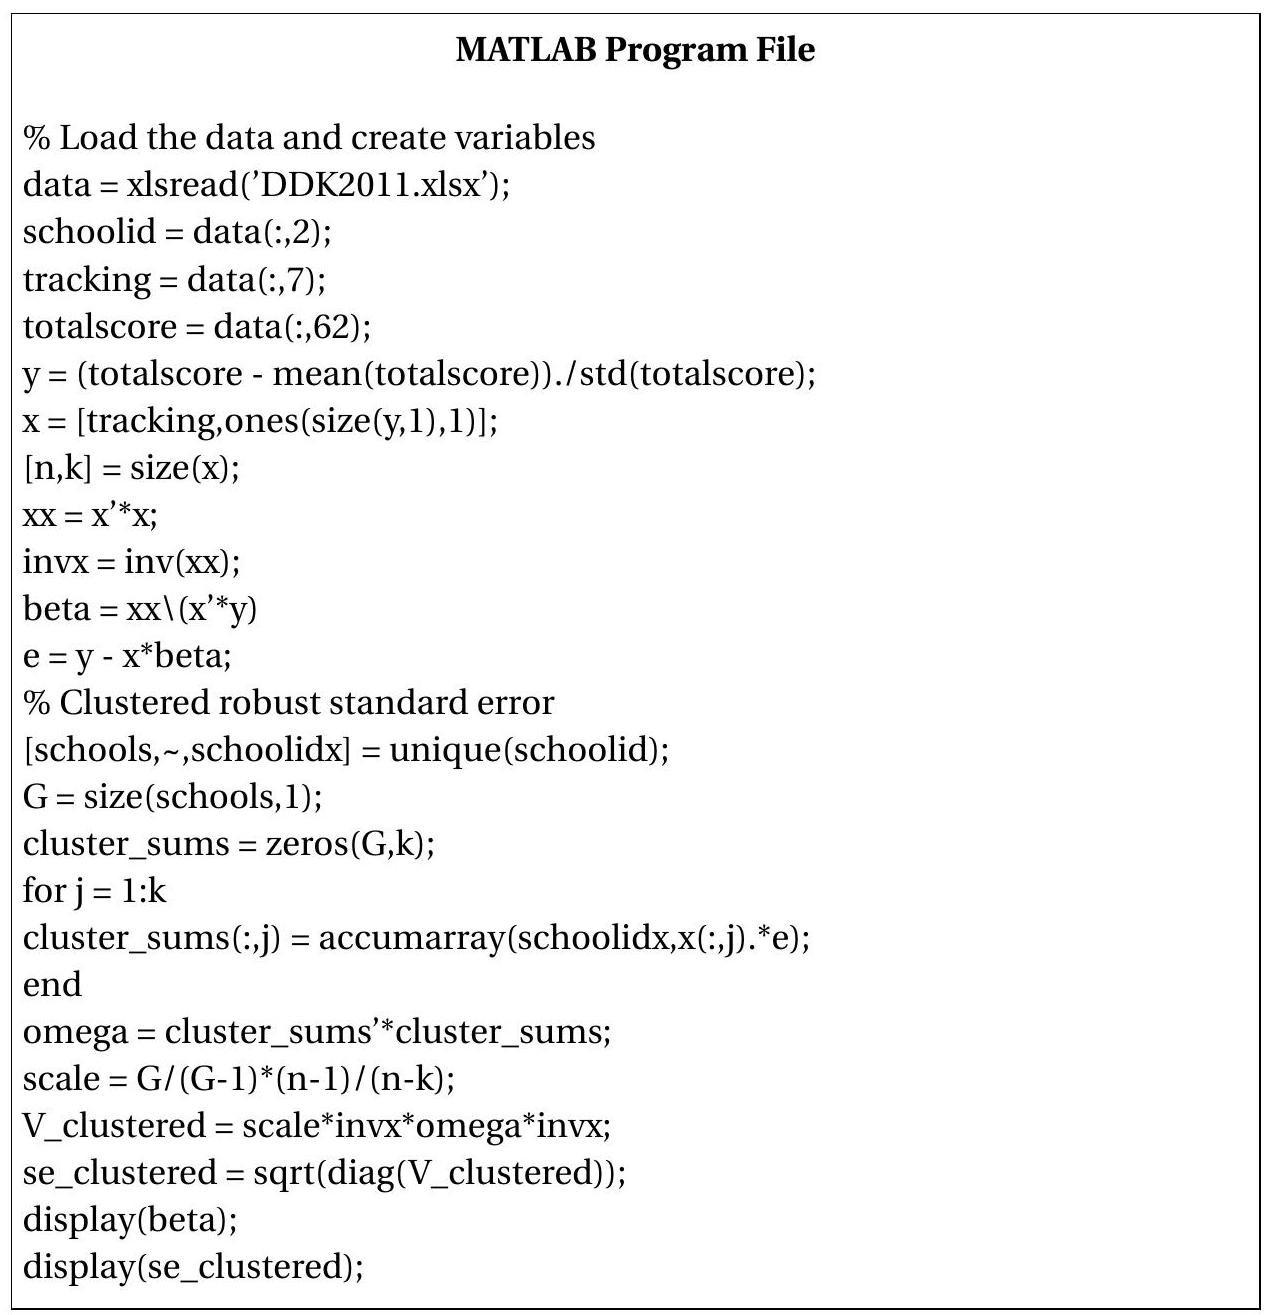
\includegraphics[max width=\textwidth]{2022_09_17_46fafb30295495354ae2g-33}

Here we see that programming clustered standard errors in MATLAB is less convenient than the other packages but still can be executed with just a few lines of code. This example uses the accumarray command which is similar to the rowsum command in $\mathrm{R}$ but only can be applied to vectors (hence the loop across the regressors) and works best if the clusterid variable are indices (which is why the original schoolid variable is transformed into indices in schoolidx. Application of these commands requires care and attention.

\subsection{Inference with Clustered Samples}
In this section we give some cautionary remarks and general advice about cluster-robust inference in econometric practice. There has been remarkably little theoretical research about the properties of cluster-robust methods - until quite recently - so these remarks may become dated rather quickly.

In many respects cluster-robust inference should be viewed similarly to heteroskedaticity-robust inference where a "cluster" in the cluster-robust case is interpreted similarly to an "observation" in the heteroskedasticity-robust case. In particular, the effective sample size should be viewed as the number of clusters, not the "sample size" $n$. This is because the cluster-robust covariance matrix estimator effectively treats each cluster as a single observation and estimates the covariance matrix based on the variation across cluster means. Hence if there are only $G=50$ clusters inference should be viewed as (at best) similar to heteroskedasticity-robust inference with $n=50$ observations. This is a bit unsettling when the number of regressors is large (say $k=20$ ) for then the covariance matrix will be estimated imprecisely.

Furthermore, most cluster-robust theory (for example, the work of Chris Hansen (2007)) assumes that the clusters are homogeneous including the assumption that the cluster sizes are all identical. This turns out to be a very important simplication. When this is violated - when, for example, cluster sizes are highly heterogeneous - the regression should be viewed as roughly equivalent to the heteroskedastic case with an extremely high degree of heteroskedasticity. Cluster sums have variances which are proportional to the cluster sizes so if the latter is heterogeneous so will be the variances of the cluster sums. This also has a large effect on finite sample inference. When clusters are heterogeneous then cluster-robust inference is similar to heteroskedasticity-robust inference with highly heteroskedastic observations.

Put together, if the number of clusters $G$ is small and the number of observations per cluster is highly varied then we should interpret inferential statements with a great degree of caution. Unfortunately, small $G$ with heterogeneous cluster sizes is commonplace. Many empirical studies on U.S. data cluster at the "state" level meaning that there are 50 or 51 clusters (the District of Columbia is typically treated as a state). The number of observations vary considerably across states since the populations are highly unequal. Thus when you read empirical papers with individual-level data but clustered at the "state" level you should be cautious and recognize that this is equivalent to inference with a small number of extremely heterogeneous observations.

A further complication occurs when we are interested in treatment as in the tracking example given in the previous section. In many cases (including Duflo, Dupas, and Kremer (2011)) the interest is in the effect of a treatment applied at the cluster level (e.g., schools). In many cases (not, however, Duflo, Dupas, and Kremer (2011)), the number of treated clusters is small relative to the total number of clusters; in an extreme case there is just a single treated cluster. Based on the reasoning given above these applications should be interpreted as equivalent to heteroskedasticity-robust inference with a sparse dummy variable as discussed in Section 4.16. As discussed there, standard error estimates can be erroneously small. In the extreme of a single treated cluster (in the example, if only a single school was tracked) then the estimated coefficient on tracking will be very imprecisely estimated yet will have a misleadingly small cluster standard error. In general, reported standard errors will greatly understate the imprecision of parameter estimates.

\subsection{At What Level to Cluster?}
A practical question which arises in the context of cluster-robust inference is "At what level should we cluster?" In some examples you could cluster at a very fine level, such as families or classrooms, or at higher levels of aggregation, such as neighborhoods, schools, towns, counties, or states. What is the correct level at which to cluster? Rules of thumb have been advocated by practitioners but at present there is little formal analysis to provide useful guidance. What do we know?

First, suppose cluster dependence is ignored or imposed at too fine a level (e.g. clustering by households instead of villages). Then variance estimators will be biased as they will omit covariance terms. As correlation is typically positive, this suggests that standard errors will be too small giving rise to spurious indications of significance and precision.

Second, suppose cluster dependence is imposed at too aggregate a measure (e.g. clustering by states rather than villages). This does not cause bias. But the variance estimators will contain many extra components so the precision of the covariance matrix estimator will be poor. This means that reported standard errors will be imprecise - more random - than if clustering had been less aggregate.

These considerations show that there is a trade-off between bias and variance in the estimation of the covariance matrix by cluster-robust methods. It is not at all clear-based on current theory - what to do. I state this emphatically. We really do not know what is the "correct" level at which to do cluster-robust inference. This is a very interesting question and should certainly be explored by econometric research. One challenge is that in empirical practice many people have observed: "Clustering is important. Standard errors change a lot whether or not we cluster. Therefore we should only report clustered standard errors." The flaw in this reasoning is that we do not know why in a specific empirical example the standard errors change under clustering. One possibility is that clustering reduces bias and thus is more accurate. The other possibility is that clustering adds sampling noise and is thus less accurate. In reality it is likely that both factors are present.

In any event a researcher should be aware of the number of clusters used in the reported calculations and should treat the number of clusters as the effective sample size for assessing inference. If the number of clusters is, say, $G=20$, this should be treated as a very small sample.

To illustrate the thought experiment consider the empirical example of Duflo, Dupas, and Kremer (2011). They reported standard errors clustered at the school level and the application uses 111 schools. Thus $G=111$ is the effective sample size. The number of observations (students) ranges from 19 to 62 , which is reasonably homogeneous. This seems like a well balanced application of clustered variance estimation. However, one could imagine clustering at a different level of aggregation. We might consider clustering at a less aggregate level such as the classroom level, but this cannot be done in this particular application as there was only one classroom per school. Clustering at a more aggregate level could be done in this application at the level of the "zone". However, there are only 9 zones. Thus if we cluster by zone, $G=9$ is the effective sample size which would lead to imprecise standard errors. In this particular example clustering at the school level (as done by the authors) is indeed the prudent choice.

\subsection{Technical Proofs*}
Proof of Theorems $\mathbf{4 . 4}$ and $\mathbf{4 . 5}$ Theorem $4.4$ is a special case so we focus on Theorem 4.5. This argument is taken from B. E. Hansen (2021).

Our approach is to calculate the Cramér-Rao bound for a carefully crafted parametric model. This is based on an insight of Newey (1990, Appendix B) for the simpler context of a population expectation.

Without loss of generality, assume that the true coefficient equals $\beta_{0}=0$ and that $\sigma^{2}=1$. These are merely normalizations which simplify the notation. Also assume that $\boldsymbol{Y}$ has a joint density $f(\boldsymbol{y})$. This assumption can be avoided through use of the Radon-Nikodym derivative.

Define the truncation function $\mathbb{R}^{n} \rightarrow \mathbb{R}^{n}$
$$
\psi_{c}(\boldsymbol{y})=\boldsymbol{y} \mathbb{1}\left\{\left|\boldsymbol{X}^{\prime} \Sigma^{-1} \boldsymbol{y}\right| \leq c\right\}-\mathbb{E}\left[\boldsymbol{Y} \mathbb{1}\left\{\left|\boldsymbol{X}^{\prime} \Sigma^{-1} \boldsymbol{Y}\right| \leq c\right\}\right] .
$$
Notice that it satisfies $\left|\psi_{c}(\boldsymbol{y})\right| \leq 2 c, \mathbb{E}\left[\psi_{c}(\boldsymbol{Y})\right]=0$, and
$$
\mathbb{E}\left[\boldsymbol{Y} \psi_{c}(\boldsymbol{Y})^{\prime}\right]=\mathbb{E}\left[\boldsymbol{Y} \boldsymbol{Y}^{\prime} \mathbb{1}\left\{\left|\boldsymbol{X}^{\prime} \Sigma^{-1} \boldsymbol{Y}\right| \leq c\right\}\right] \stackrel{\text { def }}{=} \Sigma_{c} .
$$
As $c \rightarrow \infty, \Sigma_{c} \rightarrow \mathbb{E}\left[\boldsymbol{Y} \boldsymbol{Y}^{\prime}\right]=\Sigma$. Pick $c$ sufficiently large so that $\Sigma_{c}>0$, which is feasible because $\Sigma>0$.

Define the auxiliary joint density function
$$
f_{\beta}(\boldsymbol{y})=f(\boldsymbol{y})\left(1+\psi_{c}(\boldsymbol{y})^{\prime} \Sigma_{c}^{-1} \boldsymbol{X} \beta\right)
$$
for parameters $\beta$ in the set
$$
B=\left\{\beta \in \mathbb{R}^{m}:\|\beta\| \leq \frac{1}{2 c}\right\} .
$$
The bounds imply that for $\beta \in B$ and all $y$
$$
\left|\psi_{c}(\boldsymbol{y})^{\prime} \Sigma_{c}^{-1} \boldsymbol{X} \beta\right|<1 .
$$
This implies that $f_{\beta}$ has the same support as $f$ and satisfies the bounds
$$
0<f_{\beta}(y)<2 f(y) .
$$
We calculate that
$$
\begin{aligned}
\int f_{\beta}(\boldsymbol{y}) d \boldsymbol{y} &=\int f(\boldsymbol{y}) d \boldsymbol{y}+\int \psi_{c}(\boldsymbol{y})^{\prime} \Sigma_{c}^{-1} \boldsymbol{X} \beta f_{\beta}(\boldsymbol{y}) d \boldsymbol{y} \\
&=1+\mathbb{E}\left[\psi_{c}(\boldsymbol{Y})\right]^{\prime} \Sigma_{c}^{-1} \boldsymbol{X} \beta \\
&=1
\end{aligned}
$$
the last equality because $\mathbb{E}\left[\psi_{c}(\boldsymbol{Y})\right]=0$. Together, these facts imply that $f_{\beta}$ is a valid density function, and over $\beta \in B$ is a parametric family for $\boldsymbol{Y}$. Evaluated at $\beta_{0}=0$, which is in the interior of $B$, we see $f_{0}=f$. This means that $f_{\beta}$ is a correctly-specified parametric family with the true parameter value $\beta_{0}$.

Let $\mathbb{E}_{\beta}$ denote expectation under the density $f_{\beta}$. The expectation of $\boldsymbol{Y}$ in this model is
$$
\begin{aligned}
\mathbb{E}_{\beta}[\boldsymbol{Y}] &=\int \boldsymbol{y} f_{\beta}(\boldsymbol{y}) d \boldsymbol{y} \\
&=\int \boldsymbol{y} f(\boldsymbol{y}) d \boldsymbol{y}+\int \boldsymbol{y} \psi_{c}(\boldsymbol{y})^{\prime} \Sigma_{c}^{-1} \boldsymbol{X} \beta f_{\beta}(\boldsymbol{y}) d \boldsymbol{y} \\
&=\mathbb{E}[\boldsymbol{Y}]+\mathbb{E}\left[\boldsymbol{Y} \psi_{c}(\boldsymbol{Y})^{\prime}\right] \Sigma_{c}^{-1} \boldsymbol{X} \beta \\
&=\boldsymbol{X} \beta
\end{aligned}
$$
because $\mathbb{E}[\boldsymbol{Y}]=0$ and $\mathbb{E}\left[\boldsymbol{Y}_{c}(\boldsymbol{Y})^{\prime}\right]=\Sigma_{c}$. Thus, the model $f_{\beta}$ is a linear regression with regression coefficient $\beta$.

The bound (4.61) implies
$$
\mathbb{E}_{\beta}\left[\|\boldsymbol{Y}\|^{2}\right]=\int\|\boldsymbol{y}\|^{2} f_{\beta}(\boldsymbol{y}) d \boldsymbol{y} \leq 2 \int\|\boldsymbol{y}\|^{2} f(\boldsymbol{y}) d \boldsymbol{y}=2 \mathbb{E}\left[\|\boldsymbol{Y}\|^{2}\right]=2 \operatorname{tr}(\Sigma)<\infty .
$$
This means that $f_{\beta}$ has a finite variance for all $\beta \in B$.

The likelihood score for $f_{\beta}$ is
$$
\begin{aligned}
S &=\left.\frac{\partial}{\partial \beta} \log f_{\beta}(\boldsymbol{Y})\right|_{\beta=0} \\
&=\left.\frac{\partial}{\partial \beta} \log \left(1+\psi_{c}(\boldsymbol{Y})^{\prime} \Sigma_{c}^{-1} \boldsymbol{X} \beta\right)\right|_{\beta=0} \\
&=\boldsymbol{X}^{\prime} \Sigma_{c}^{-1} \psi_{c}(\boldsymbol{Y}) .
\end{aligned}
$$
The information matrix is
$$
\begin{aligned}
\mathscr{I}_{c} &=\mathbb{E}\left[S S^{\prime}\right] \\
&=\boldsymbol{X}^{\prime} \Sigma_{c}^{-1} \mathbb{E}\left[\psi_{c}(\boldsymbol{Y}) \psi_{c}(\boldsymbol{Y})^{\prime}\right] \Sigma_{c}^{-1} \boldsymbol{X} \\
& \leq \boldsymbol{X}^{\prime} \Sigma_{c}^{-1} \boldsymbol{X},
\end{aligned}
$$
where the inequality is
$$
\mathbb{E}\left[\psi_{c}(\boldsymbol{Y}) \psi_{c}(\boldsymbol{Y})^{\prime}\right]=\Sigma_{c}-\mathbb{E}\left[\boldsymbol{Y} \mathbb{1}\left\{\left|\boldsymbol{X}^{\prime} \Sigma^{-1} \boldsymbol{Y}\right| \leq c\right\}\right] \mathbb{E}\left[\boldsymbol{Y} \mathbb{1}\left\{\left|\boldsymbol{X}^{\prime} \Sigma^{-1} \boldsymbol{Y}\right| \leq c\right\}\right]^{\prime} \leq \Sigma_{c} .
$$
By assumption, the estimator $\widetilde{\beta}$ is unbiased for $\beta$. The model $f_{\beta}$ is regular (it is correctly specified as it contains the true density $f$, the support of $Y$ does not depend on $\beta$, and the true value $\beta_{0}=0$ lies in the interior of $B$ ). Thus by the Cramér-Rao Theorem (Theorem $10.6$ of Probability and Statistics for Economists)
$$
\operatorname{var}[\widetilde{\beta}] \geq \mathscr{I}_{c}^{-1} \geq\left(\boldsymbol{X}^{\prime} \Sigma_{c}^{-1} \boldsymbol{X}\right)^{-1}
$$
where the second inequality is (4.62). Since this holds for all $c$, and $\Sigma_{c} \rightarrow \Sigma$ as $c \rightarrow \infty$,
$$
\operatorname{var}[\widetilde{\beta}] \geq \limsup _{c \rightarrow \infty}\left(\boldsymbol{X}^{\prime} \Sigma_{c}^{-1} \boldsymbol{X}\right)^{-1}=\left(\boldsymbol{X}^{\prime} \Sigma^{-1} \boldsymbol{X}\right)^{-1} .
$$
This is the variance lower bound.

\section{$4.25$ Exercises}
Exercise 4.1 For some integer $k$, set $\mu_{k}=\mathbb{E}\left[Y^{k}\right]$.

(a) Construct an estimator $\widehat{\mu}_{k}$ for $\mu_{k}$.

(b) Show that $\widehat{\mu}_{k}$ is unbiased for $\mu_{k}$.

(c) Calculate the variance of $\widehat{\mu}_{k}$, say $\operatorname{var}\left[\widehat{\mu}_{k}\right]$. What assumption is needed for $\operatorname{var}\left[\widehat{\mu}_{k}\right]$ to be finite?

(d) Propose an estimator of $\operatorname{var}\left[\widehat{\mu}_{k}\right]$

Exercise 4.2 Calculate $\mathbb{E}\left[(\bar{Y}-\mu)^{3}\right]$, the skewness of $\bar{Y}$. Under what condition is it zero?

Exercise 4.3 Explain the difference between $\bar{Y}$ and $\mu$. Explain the difference between $n^{-1} \sum_{i=1}^{n} X_{i} X_{i}^{\prime}$ and $\mathbb{E}\left[X_{i} X_{i}^{\prime}\right]$

Exercise 4.4 True or False. If $Y=X^{\prime} \beta+e, X \in \mathbb{R}, \mathbb{E}[e \mid X]=0$, and $\widehat{e}_{i}$ is the OLS residual from the regression of $Y_{i}$ on $X_{i}$, then $\sum_{i=1}^{n} X_{i}^{2} \widehat{e}_{i}=0$.

Exercise 4.5 Prove (4.20) and (4.21).

Exercise 4.6 Prove Theorem $4.5$ under the restriction to linear estimators.

Exercise 4.7 Let $\widetilde{\beta}$ be the GLS estimator (4.22) under the assumptions (4.18) and (4.19). Assume that $\Sigma$ is known and $\sigma^{2}$ is fdunknown. Define the residual vector $\widetilde{\boldsymbol{e}}=\boldsymbol{Y}-\boldsymbol{X} \widetilde{\beta}$, and an estimator for $\sigma^{2}$
$$
\widetilde{\sigma}^{2}=\frac{1}{n-k} \widetilde{\boldsymbol{e}}^{\prime} \Sigma^{-1} \widetilde{\boldsymbol{e}}
$$
(a) Show (4.23).

(b) Show (4.24).

(c) Prove that $\widetilde{\boldsymbol{e}}=\boldsymbol{M}_{1} \boldsymbol{e}$, where $\boldsymbol{M}_{1}=\boldsymbol{I}-\boldsymbol{X}\left(\boldsymbol{X}^{\prime} \Sigma^{-1} \boldsymbol{X}\right)^{-1} \boldsymbol{X}^{\prime} \Sigma^{-1}$.

(d) Prove that $\boldsymbol{M}_{1}^{\prime} \Sigma^{-1} \boldsymbol{M}_{1}=\Sigma^{-1}-\Sigma^{-1} \boldsymbol{X}\left(\boldsymbol{X}^{\prime} \Sigma^{-1} \boldsymbol{X}\right)^{-1} \boldsymbol{X}^{\prime} \Sigma^{-1}$. (e) Find $\mathbb{E}\left[\widetilde{\sigma}^{2} \mid \boldsymbol{X}\right]$.

(f) Is $\widetilde{\sigma}^{2}$ a reasonable estimator for $\sigma^{2}$ ?

Exercise 4.8 Let $\left(Y_{i}, X_{i}\right)$ be a random sample with $\mathbb{E}[Y \mid X]=X^{\prime} \beta$. Consider the Weighted Least Squares (WLS) estimator $\widetilde{\beta}_{\text {wls }}=\left(\boldsymbol{X}^{\prime} \boldsymbol{W} \boldsymbol{X}\right)^{-1}\left(\boldsymbol{X}^{\prime} \boldsymbol{W} \boldsymbol{Y}\right)$ where $\boldsymbol{W}=\operatorname{diag}\left(w_{1}, \ldots, w_{n}\right)$ and $w_{i}=X_{j i}^{-2}$, where $X_{j i}$ is one of the $X_{i}$.

(a) In which contexts would $\widetilde{\beta}_{\mathrm{wls}}$ be a good estimator?

(b) Using your intuition, in which situations do you expect $\widetilde{\beta}_{\text {wls }}$ to perform better than OLS?

Exercise 4.9 Show (4.32) in the homoskedastic regression model.

Exercise 4.10 Prove (4.40).

Exercise 4.11 Show (4.41) in the homoskedastic regression model.

Exercise 4.12 Let $\mu=\mathbb{E}[Y], \sigma^{2}=\mathbb{E}\left[(Y-\mu)^{2}\right]$ and $\mu_{3}=\mathbb{E}\left[(Y-\mu)^{3}\right]$ and consider the sample mean $\bar{Y}=$ $\frac{1}{n} \sum_{i=1}^{n} Y_{i}$. Find $\mathbb{E}\left[(\bar{Y}-\mu)^{3}\right]$ as a function of $\mu, \sigma^{2}, \mu_{3}$ and $n$.

Exercise 4.13 Take the simple regression model $Y=X \beta+e, X \in \mathbb{R}, \mathbb{E}[e \mid X]=0$. Define $\sigma_{i}^{2}=\mathbb{E}\left[e_{i}^{2} \mid X_{i}\right]$ and $\mu_{3 i}=\mathbb{E}\left[e_{i}^{3} \mid X_{i}\right]$ and consider the OLS coefficient $\widehat{\beta}$. Find $\mathbb{E}\left[(\widehat{\beta}-\beta)^{3} \mid \boldsymbol{X}\right]$.

Exercise 4.14 Take a regression model $Y=X \beta+e$ with $\mathbb{E}[e \mid X]=0$ and i.i.d. observations $\left(Y_{i}, X_{i}\right)$ and scalar $X$. The parameter of interest is $\theta=\beta^{2}$. Consider the OLS estimators $\widehat{\beta}$ and $\widehat{\theta}=\widehat{\beta}^{2}$.

(a) Find $\mathbb{E}[\widehat{\theta} \mid \boldsymbol{X}]$ using our knowledge of $\mathbb{E}[\widehat{\beta} \mid \boldsymbol{X}]$ and $V_{\widehat{\beta}}=\operatorname{var}[\widehat{\beta} \mid \boldsymbol{X}]$. Is $\widehat{\theta}$ biased for $\theta$ ?

(b) Suggest an (approximate) biased-corrected estimator $\widehat{\theta}^{*}$ using an estimator $\widehat{V}_{\widehat{\beta}}$ for $V_{\widehat{\beta}}$.

(c) For $\widehat{\theta}^{*}$ to be potentially unbiased, which estimator of $V_{\widehat{\beta}}$ is most appropriate?

Under which conditions is $\widehat{\theta}^{*}$ unbiased?

Exercise 4.15 Consider an i.i.d. sample $\left\{Y_{i}, X_{i}\right\} i=1, \ldots, n$ where $X$ is $k \times 1$. Assume the linear conditional expectation model $Y=X^{\prime} \beta+e$ with $\mathbb{E}[e \mid X]=0$. Assume that $n^{-1} \boldsymbol{X}^{\prime} \boldsymbol{X}=\boldsymbol{I}_{k}$ (orthonormal regressors). Consider the OLS estimator $\widehat{\beta}$.

(a) Find $\boldsymbol{V}_{\widehat{\beta}}=\operatorname{var}[\widehat{\beta}]$

(b) In general, are $\widehat{\beta}_{j}$ and $\widehat{\beta}_{\ell}$ for $j \neq \ell$ correlated or uncorrelated?

(c) Find a sufficient condition so that $\widehat{\beta}_{j}$ and $\widehat{\beta}_{\ell}$ for $j \neq \ell$ are uncorrelated.

Exercise 4.16 Take the linear homoskedastic CEF
$$
\begin{aligned}
Y^{*} &=X^{\prime} \beta+e \\
\mathbb{E}[e \mid X] &=0 \\
\mathbb{E}\left[e^{2} \mid X\right] &=\sigma^{2}
\end{aligned}
$$
and suppose that $Y^{*}$ is measured with error. Instead of $Y^{*}$, we observe $Y=Y^{*}+u$ where $u$ is measurement error. Suppose that $e$ and $u$ are independent and
$$
\begin{aligned}
\mathbb{E}[u \mid X] &=0 \\
\mathbb{E}\left[u^{2} \mid X\right] &=\sigma_{u}^{2}(X)
\end{aligned}
$$
(a) Derive an equation for $Y$ as a function of $X$. Be explicit to write the error term as a function of the structural errors $e$ and $u$. What is the effect of this measurement error on the model (4.63)?

(b) Describe the effect of this measurement error on OLS estimation of $\beta$ in the feasible regression of the observed $Y$ on $X$.

(c) Describe the effect (if any) of this measurement error on standard error calculation for $\widehat{\beta}$.

Exercise 4.17 Suppose that for the random variables $(Y, X)$ with $X>0$ an economic model implies
$$
\mathbb{E}[Y \mid X]=(\gamma+\theta X)^{1 / 2} .
$$
A friend suggests that you estimate $\gamma$ and $\theta$ by the linear regression of $Y^{2}$ on $X$, that is, to estimate the equation
$$
Y^{2}=\alpha+\beta X+e .
$$
(a) Investigate your friend's suggestion. Define $u=Y-(\gamma+\theta X)^{1 / 2}$. Show that $\mathbb{E}[u \mid X]=0$ is implied by (4.64).

(b) Use $Y=(\gamma+\theta X)^{1 / 2}+u$ to calculate $\mathbb{E}\left[Y^{2} \mid X\right]$. What does this tell you about the implied equation (4.65)?

(c) Can you recover either $\gamma$ and/or $\theta$ from estimation of (4.65)? Are additional assumptions required?

(d) Is this a reasonable suggestion?

Exercise 4.18 Take the model
$$
\begin{aligned}
Y &=X_{1}^{\prime} \beta_{1}+X_{2}^{\prime} \beta_{2}+e \\
\mathbb{E}[e \mid X] &=0 \\
\mathbb{E}\left[e^{2} \mid X\right] &=\sigma^{2}
\end{aligned}
$$
where $X=\left(X_{1}, X_{2}\right)$, with $X_{1} k_{1} \times 1$ and $X_{2} k_{2} \times 1$. Consider the short regression $Y_{i}=X_{1 i}^{\prime} \widehat{\beta}_{1}+\widehat{e}_{i}$ and define the error variance estimator $s^{2}=\left(n-k_{1}\right)^{-1} \sum_{i=1}^{n} \widehat{e}_{i}^{2}$. Find $\mathbb{E}\left[s^{2} \mid \boldsymbol{X}\right]$.

Exercise 4.19 Let $\boldsymbol{Y}$ be $n \times 1, \boldsymbol{X}$ be $n \times k$, and $\boldsymbol{X}^{*}=\boldsymbol{X} \boldsymbol{C}$ where $\boldsymbol{C}$ is $k \times k$ and full-rank. Let $\widehat{\beta}$ be the least squares estimator from the regression of $Y$ on $X$, and let $\widehat{V}$ be the estimate of its asymptotic covariance matrix. Let $\widehat{\beta}^{*}$ and $\widehat{\boldsymbol{V}}^{*}$ be those from the regression of $\boldsymbol{Y}$ on $\boldsymbol{X}^{*}$. Derive an expression for $\widehat{\boldsymbol{V}}^{*}$ as a function of $\widehat{V}$.

Exercise 4.20 Take the model in vector notation
$$
\begin{aligned}
\boldsymbol{Y} &=\boldsymbol{X} \beta+\boldsymbol{e} \\
\mathbb{E}[\boldsymbol{e} \mid \boldsymbol{X}] &=0 \\
\mathbb{E}\left[\boldsymbol{e} \boldsymbol{e}^{\prime} \mid \boldsymbol{X}\right] &=\Sigma .
\end{aligned}
$$
Assume for simplicity that $\Sigma$ is known. Consider the OLS and GLS estimators $\widehat{\beta}=\left(\boldsymbol{X}^{\prime} \boldsymbol{X}\right)^{-1}\left(\boldsymbol{X}^{\prime} \boldsymbol{Y}\right)$ and $\widetilde{\beta}=\left(\boldsymbol{X}^{\prime} \Sigma^{-1} \boldsymbol{X}\right)^{-1}\left(\boldsymbol{X}^{\prime} \Sigma^{-1} \boldsymbol{Y}\right)$. Compute the (conditional) covariance between $\widehat{\beta}$ and $\widetilde{\beta}$ :
$$
\mathbb{E}\left[(\widehat{\beta}-\beta)(\widetilde{\beta}-\beta)^{\prime} \mid \boldsymbol{X}\right]
$$
Find the (conditional) covariance matrix for $\widehat{\beta}-\widetilde{\beta}$ :
$$
\mathbb{E}\left[(\widehat{\beta}-\widetilde{\beta})(\widehat{\beta}-\beta)^{\prime} \mid \boldsymbol{X}\right] .
$$
Exercise 4.21 The model is
$$
\begin{aligned}
Y_{i} &=X_{i}^{\prime} \beta+e_{i} \\
\mathbb{E}\left[e_{i} \mid X_{i}\right] &=0 \\
\mathbb{E}\left[e_{i}^{2} \mid X_{i}\right] &=\sigma_{i}^{2} \\
\Sigma &=\operatorname{diag}\left\{\sigma_{1}^{2}, \ldots, \sigma_{n}^{2}\right\} .
\end{aligned}
$$
The parameter $\beta$ is estimated by OLS $\widehat{\beta}=\left(\boldsymbol{X}^{\prime} \boldsymbol{X}\right)^{-1} \boldsymbol{X}^{\prime} \boldsymbol{Y}$ and GLS $\widetilde{\beta}=\left(\boldsymbol{X}^{\prime} \Sigma^{-1} \boldsymbol{X}\right)^{-1} \boldsymbol{X}^{\prime} \Sigma^{-1} \boldsymbol{Y}$. Let $\widehat{\boldsymbol{e}}=\boldsymbol{Y}-\boldsymbol{X} \widehat{\beta}$ and $\widetilde{\boldsymbol{e}}=\boldsymbol{Y}-\boldsymbol{X} \widetilde{\beta}$ denote the residuals. Let $\widehat{R}^{2}=1-\widehat{\boldsymbol{e}}^{\prime} \widehat{\boldsymbol{e}} /\left(\boldsymbol{Y}^{* \prime} \boldsymbol{Y}^{*}\right)$ and $\widetilde{R}^{2}=1-\widetilde{\boldsymbol{e}}^{\prime} \widetilde{\boldsymbol{e}} /\left(\boldsymbol{Y}^{* \prime} \boldsymbol{Y}^{*}\right)$ denote the equation $R^{2}$ where $\boldsymbol{Y}^{*}=\boldsymbol{Y}-\bar{Y}$. If the error $e_{i}$ is truly heteroskedastic will $\widehat{R}^{2}$ or $\widetilde{R}^{2}$ be smaller?

Exercise 4.22 An economist friend tells you that the assumption that the observations $\left(Y_{i}, X_{i}\right)$ are i.i.d. implies that the regression $Y=X^{\prime} \beta+e$ is homoskedastic. Do you agree with your friend? How would you explain your position?

Exercise 4.23 Take the linear regression model with $\mathbb{E}[\boldsymbol{Y} \mid \boldsymbol{X}]=\boldsymbol{X} \beta$. Define the ridge regression estimator
$$
\widehat{\beta}=\left(\boldsymbol{X}^{\prime} \boldsymbol{X}+\boldsymbol{I}_{k} \lambda\right)^{-1} \boldsymbol{X}^{\prime} \boldsymbol{Y}
$$
where $\lambda>0$ is a fixed constant. Find $E[\widehat{\beta} \mid \boldsymbol{X}]$. Is $\widehat{\beta}$ biased for $\beta$ ?

Exercise 4.24 Continue the empirical analysis in Exercise 3.24.

(a) Calculate standard errors using the homoskedasticity formula and using the four covariance matrices from Section $4.14 .$

(b) Repeat in a second programming language. Are they identical?

Exercise 4.25 Continue the empirical analysis in Exercise 3.26. Calculate standard errors using the HC3 method. Repeat in your second programming language. Are they identical?

Exercise 4.26 Extend the empirical analysis reported in Section $4.21$ using the DDK2011 dataset on the textbook website.. Do a regression of standardized test score (totalscore normalized to have zero mean and variance 1) on tracking, age, gender, being assigned to the contract teacher, and student's percentile in the initial distribution. (The sample size will be smaller as some observations have missing variables.) Calculate standard errors using both the conventional robust formula, and clustering based on the school.

(a) Compare the two sets of standard errors. Which standard error changes the most by clustering? Which changes the least?

(b) How does the coefficient on tracking change by inclusion of the individual controls (in comparison to the results from (4.60))?


\end{document}